\documentclass{article}

%%%%%%%%%%%%%%%%%%%%%%%%%%%%%%%%%%%%%%%%%%%%%%%%%%%%%%%%
% LATEX DEFINITIONS 
%%%%%%%%%%%%%%%%%%%%%%%%%%%%%%%%%%%%%%%%%%%%%%%%%%%%%%%%

\usepackage{enumerate}
\usepackage{hyperref}
\usepackage{array}
\usepackage{graphicx}
\usepackage{booktabs}
\usepackage{pifont}
\usepackage{todonotes}
\usepackage{rotating}
\usepackage{color}
\usepackage{afterpage}
\usepackage{amssymb}
\usepackage{latexsym}

\newcommand*\rot{\rotatebox{90}}

%\newcommand{\FILE}[1]{\todo[color=green!40]{#1}}


\newcommand{\FILE}[1]{}

%%%%%%%%%%%%%%%%%%%%%%%%%%%%%%%%%%%%%%%%%%%%%%%%%%%%%%%%
% TITLE ABLE OF CONTENTS
%%%%%%%%%%%%%%%%%%%%%%%%%%%%%%%%%%%%%%%%%%%%%%%%%%%%%%%%

\newcommand{\TITLE}{The FutureGrid Testbed for Big Data}
\newcommand{\AUTHOR}{Gregor von Laszewsi, Geoffrey C. Fox}
\newcommand{\EMAIL}{laszewski@gmail.com}
\begin{document}

\title{\TITLE}
\author{\AUTHOR}
\date{\EMAIL}


%%%%%%%%%%%%%%%%%%%%%%%%%%%%%%%%%%%%%%%%%%%%%%%%%%%%%%%%
% TABLE OF CONTENTS
%%%%%%%%%%%%%%%%%%%%%%%%%%%%%%%%%%%%%%%%%%%%%%%%%%%%%%%%

\pagenumbering{roman}

\begin{center}
{\Large\bf \TITLE}\\
{\AUTHOR}\\
{\EMAIL}
\end{center}

\tableofcontents

\newpage

%%%%%%%%%%%%%%%%%%%%%%%%%%%%%%%%%%%%%%%%%%%%%%%%%%%%%%%%
% LIST OF TODOS
%%%%%%%%%%%%%%%%%%%%%%%%%%%%%%%%%%%%%%%%%%%%%%%%%%%%%%%%

\listoftodos

\newpage

%%%%%%%%%%%%%%%%%%%%%%%%%%%%%%%%%%%%%%%%%%%%%%%%%%%%%%%%
% TITLE OF PAPER
%%%%%%%%%%%%%%%%%%%%%%%%%%%%%%%%%%%%%%%%%%%%%%%%%%%%%%%%

\pagenumbering{arabic}

\maketitle

%%%%%%%%%%%%%%%%%%%%%%%%%%%%%%%%%%%%%%%%%%%%%%%%%%%%%%%%
% ABSTRACT OF PAPER
%%%%%%%%%%%%%%%%%%%%%%%%%%%%%%%%%%%%%%%%%%%%%%%%%%%%%%%%


\begin{abstract}

In this chapter we will be introducing you to FutureGrid that provides a testbed to conduct research for Cloud, Grid, and High Performance Computing. Although FutureGrid has only a modest number of compute cores (about 4500 regular cores and 14000 GPU cores) it provides an ideal playground to test out various frameworks that may be useful for users to consider as part of their big data analysis pipelines. We will be focusing here on the use of FutureGrid for big data related testbed research.

The chapter is structured as follows. First we will provide the reader with an introduction to Future Grid hardware (Section \ref{S:overview}).   Next we will focus on a selected number of services and tools that have been proven to be useful to conduct big data research on FutureGrid (Section \ref{S:services}). We will contrast frameworks such as MPI, virtual large memory systems, Infrastructure as a Service and map/reduce frameworks. Next we will present reasoning by analyzing requests to use certain technologies and identify trends within the user community to direct effort in FutureGrid (Section \ref{S:usage}). The next section will report on our experience with the integration of our software and systems teams via DevOps (Section \ref{S:devops}). Next we summarize cloudmesh, which is a logical continuation of the FutureGrid architecture and provides abilities to federate cloud services, but also to conduct cloudshifting, that is to assign servers on-demand to HPC and Cloud services (Section \ref{S:cloudmesh}). We conclude the chapter with a brief summary (Section \ref{S:summary}).
\end{abstract}

%%%%%%%%%%%%%%%%%%%%%%%%%%%%%%%%%%%%%%%%%%%%%%%%%%%%%%%%
% SECTIONS
%%%%%%%%%%%%%%%%%%%%%%%%%%%%%%%%%%%%%%%%%%%%%%%%%%%%%%%%

\FILE{introduction.tex}

\section{Introduction}

FutureGrid \cite{las2010gce,las12fg-bookchapter}``is a project led by Indiana University and funded by the National Science Foundation (NSF) to develop a high performance grid test bed that will allow scientists to collaboratively develop and test innovative approaches to parallel, grid, and cloud computing. FutureGrid will provide the infrastructure to researchers that allows them to perform their own computational experiments using distributed systems. The goal is to make it easier for scientists to conduct such experiments in a transparent manner.  FutureGrid users will be able to deploy their own hardware and software configurations on a public/private cloud, and run their experiments. They will be able to save their configurations and execute their experiments using the provided tools. The FutureGrid test bed is composed of a high speed network connecting distributed clusters of high performance computers. FutureGrid employs virtualization technology that will allow the test bed to support a wide range of operating systems.''



\section{Overview of FutureGrid}\label{S:overview}

\FILE{hardware.tex}

\subsection{Hardware Overview}

FutureGrid contains a number of clusters of different type and size that are interconnected with up to a 10GB Ethernet among its sites. The sites include Indiana University, University of Chicago, San Diego Supercomputing Center, Texas Advanced Computing Center, and University of Florida.

\subsubsection{Overview of the Clusters}\label{S:hw-cluster} 

Table \ref{T:hw} provides a high level overview of the clusters currently available in FutureGrid.  The biggest cluster is located at IU called India and contains 128 servers with 1024 cores. In total we have currently 481 compute servers with 1126 CPUs and 4496 Cores. In addition we also have 448 GPU cores. The total RAM is about 21.5TB. Secondary storage is about 1PB. A more detailed table is provided in Table \ref{F:cluster-details}.

\begin{table}[htb]

\caption{FutureGrid Compute Resources}\label{T:hw}

\begin{center}
\begin{tabular}{rrrrrrrrr}
Name    & System Type                &  \rot{Nodes} &  \rot{CPUS}   & \rot{Cores}   & \rot{TFLOPS}  & \rot{RAM (GB)}        & \rot{Storage (TB)}    & Site \\
\hline
india   & IBM iDataplex              & 128          & 256     & 1024    & 11      & 3072            & 335             & IU \\
hotel   & IBM iDataplex              & 84           & 168     & 672     & 7       & 2016            & 120             & UC \\
sierra  & IBM iDataplex              & 84           & 168     & 672     & 7       & 2688            & 96              & SDSC \\
foxtrot & IBM iDataplex              & 32           & 64      & 256     & 3       & 768             & 0               & UF \\
alamo   & Dell Poweredge             & 96           & 192     & 768     & 8       & 1152            & 30              & TACC \\
xray    & Cray XT5m                  & 1            & 166     & 664     & 6       & 1328            & 5.4             & IU \\
bravo   & HP Proliant                & 16           & 32      & 128     & 1.7     & 3072            & 128             & IU \\
delta   & \shortstack{SuperMicro\\ GPU Cluster}     & 16           & 32      & 192     &         & 1333            & 144             & IU \\
lima    & Aeon Eclipse64             & 8            & 16      & 128     & 1.3     & 512             & 3.8             & SDSC \\
echo    & \shortstack{SuperMicro \\ScaleMP Cluster} & 16           & 32      & 192     & 2       & 6144            & 192             & IU \\
\hline
&& 481	& 1126 & 	\footnote{GPU cores on machines not included}4696 & 47	& 22085	& 1054.2 \\
\end{tabular}
\end{center}
\end{table}


\begin{sidewaystable}

\caption{FutureGrid cluster details.}\label{F:cluster-details}
~\\
\begin{footnotesize}
\begin{tabular}{|p{2cm}||p{4cm}p{1.5cm}p{1.5cm}p{1.5cm}p{1.5cm}p{1.5cm}p{1.5cm}p{1.5cm}p{1cm}|}
\hline
 \bf Name                                & \bf Echo & \bf Alamo & \bf Bravo & \bf Delta & \bf Foxtrot & \bf Hotel & \bf India & \bf Sierra & \bf Xray \\
\hline
\hline
 Organization                        & IU & TACC & IU & IU & UF & UC & IU & SDSC & IU \\
\hline
 Machine Type                        & Cluster SclaeMP & Cluster & Cluster & Cluster & Cluster & Cluster & Cluster & Cluster & Cluster \\
\hline
 System Type                         &SuperMicro& Dell PowerEdge M610 Blade & HP Proliant && IBM iDataPlex dx 360 M2 & IBM iDataPlex dx 360 M2 & IBM iDataPlex dx 360 M2 & IBM iDataPlex dx 340 & Cray XT5m \\
\hline
 CPU Type                            & Xeon E5-2640 &  Xeon X5550 &  Xeon E5620 &  Xeon 5660 &  Xeon X5520 &  Xeon X5550 &  Xeon X5550 &  Xeon L5420 & Opteron 2378 \\
\hline
 CPU Speed                           &2.50GHz& 2.66GHz & 2.40GHz & 2.80 GHz & 2.26GHz & 2.66GHz & 2.66GHz & 2.5GHz & 2.4GHz \\
\hline
 CPUs                                &&192&32&32&64&168&256&168&168 \\
\hline
 Servers                             &12&96&16&16&32&84&128&84&1 \\
\hline
 RAM                                 && 12GB DDR3 1333Mhz & 192GB DDR3 1333Mhz & 192GB DDR3 1333 Mhz & 24GB DDR3 1333Mhz & 24GB DDR3 1333Mhz & 24GB DDR3 1333Mhz & 32GB DDR2-667 & 8GB DDR2-800 \\
\hline
 Total RAM                           &&1152GB&3072GB&3072GB&768GB&2016GB&3072GB&2688GB&1344GB \\
\hline
 Number of cores                     &144&768&128&&256&672&1024&672&672 \\
\hline
 Tflops                              &&8&1.7&&3&7&11&7&6 \\
\hline
 Disk Size (TB)                      &2.8&48&&15&20&120&335&72&335 \\
\hline
 Hard Drives                         && 500GB 7.2K RPM SAS & 6x2TB 7.2K RPM SATA & 92GB 7.2K RPM SAS2 & 500GB 7200 RPM SATA & 1 TB 7200 RPM SATA & 3000GB 7200 RPM SATA & 160GB 7200 RPM SATA Drive & 6TB Lustre \\
\hline
 Shared Storage                      && NFS & NFS &NFS& NFS & GPFS & NFS & ZFS 82.2TB & NFS \\
\hline
 Interconnect                        && Mellanox 4x QDR IB & Mellanox 4x DDR IB &&& Mellanox 4x DDR IB & Mellanox 4x DDR IB & Mellanox 4x DDR IB & Cray SeaStar \\
\hline
\end{tabular}
~\\
IB = InfiniBand, Xenon = INtel Xenon, Opteron = AMD Opteron 

\end{footnotesize}

\end{sidewaystable}



\subsubsection{Overview of Networking}

The significant number of distinct systems within FutureGrid provide a heterogeneous distributed architecture and are connected by high-bandwidth network links supporting distributed system research \cite{las12fg-bookchapter}. The FutureGrid network used to have a dedicated network between sites \cite{las12fg-bookchapter}. However, the network infrastructure has recently changed due to changes related to the its major network operator the National Lambda Rail.  Due to these changes the operation of the network between the sites has switched from the national lambda rail to XSEDE and are no longer exclusive. However, this is so far no major handicap for the projects conducted on FutureGrid based on our project portfolio.  The current high level network diagram is depicted in Figure~\ref{F:network}. Hence, the core resources to FutureGrid at SDSC, IU, TACC, and UF are now all connected via the XSEDE network and integrated via the FG core router in Chicago. Within the IU network additional clusters are integrated and are described in more detail in Section~\ref{S:hw-cluster}.

A Spirent H10 XGEM Network Impairment emulator \cite{www-network-impairment} can be collocated with resources at Indiana University, to enable experiments to include network latency, jitter, loss, and errors to network traffic. 

In addition we have added several components that are related to a special software service called cloudmesh, which we explain in more detail in Section~\ref{S:cloudmesh}. 

\begin{figure}[htb]
  \centering
    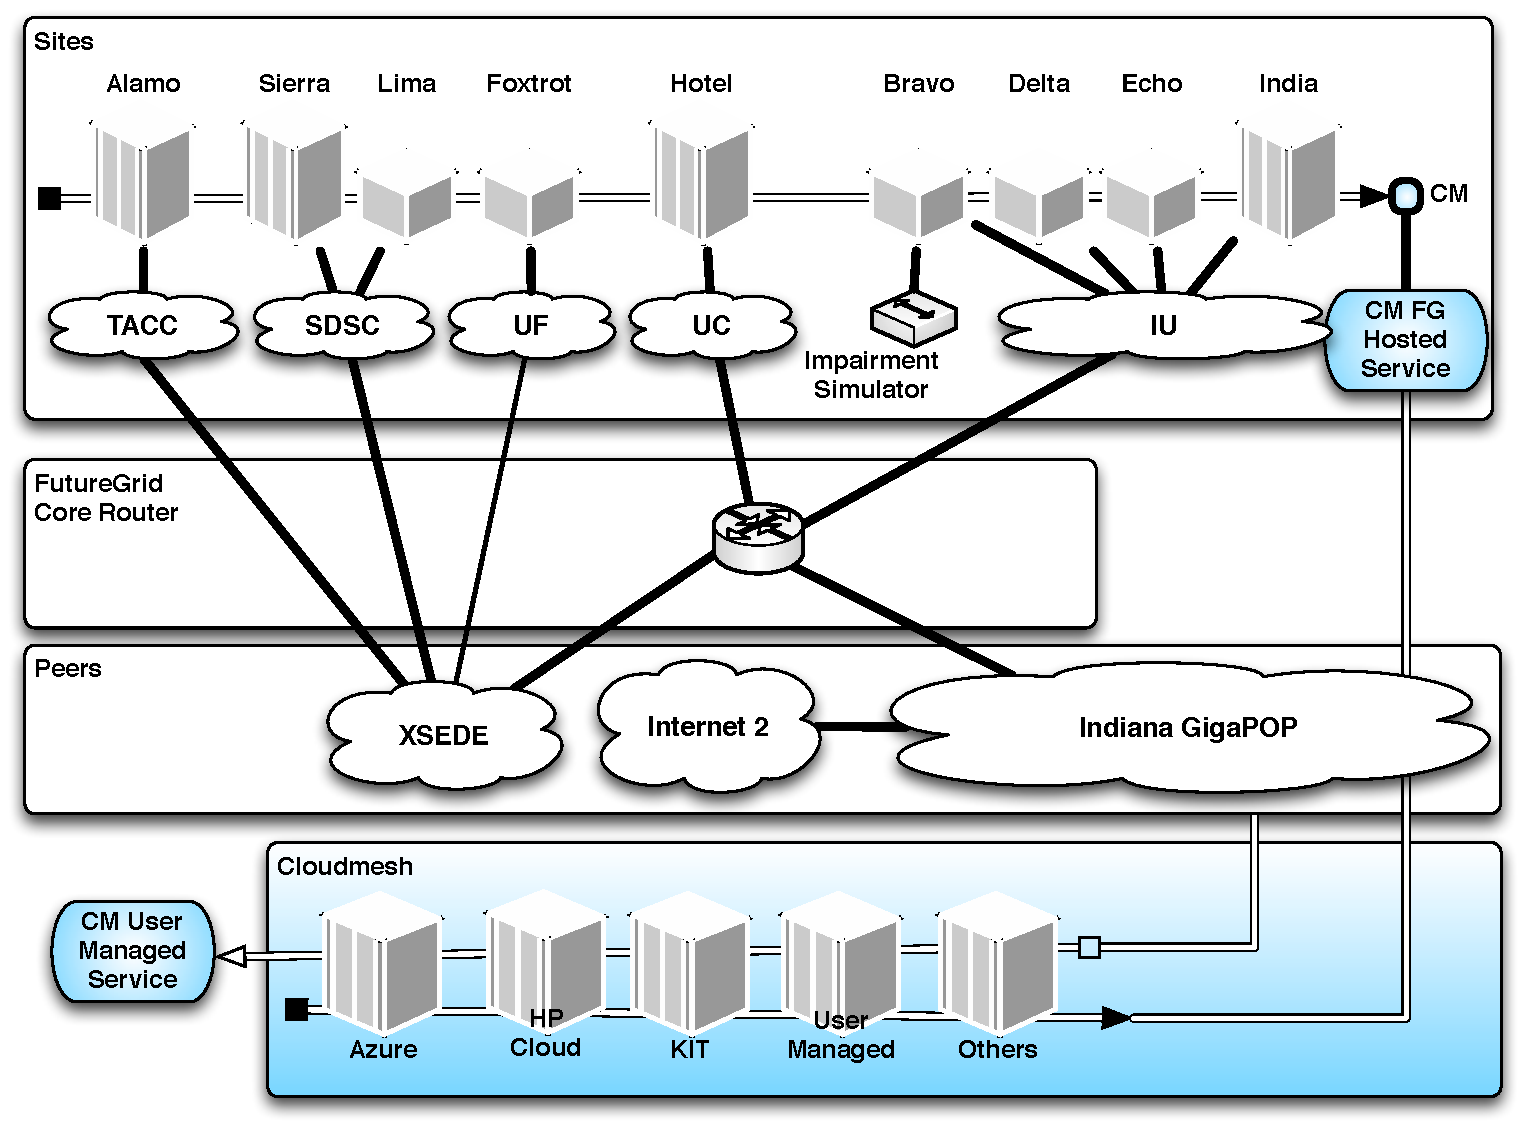
\includegraphics[width=1.0\textwidth]{images/fg-network-2014-cm.pdf}
  \caption{High level network diagram and conceptual integration of cloudmesh resources.}
\label{F:network}
\end{figure}

\subsubsection{Overview of Storage}

FutureGrid does not provide capacity for long-term storage or long-term experiments. FutureGrid has a limited amount of storage space and users are requested to remove their storage after use. However, users with special needs may be accommodated by special storage setups. The list of storage services is shown in Table \ref{T:storage}.

\begin{table}[htb]
\caption{Storage Resources of FutureGrid.}
\label{T:storage} 

\centering{}%
\begin{tabular}{lrll}
\textbf{System Type } & \textbf{Capacity(TB) } & \textbf{File System } & \textbf{Site }\tabularnewline
\hline 
Xanadu 360  & 180  & NFS  & IU \tabularnewline
DDN 6620  & 120  & GPFS  & UC \tabularnewline
Sunfire x4170  & 96  & ZFS  & SDSC \tabularnewline
Dell MD3000  & 30  & NFS  & TACC \tabularnewline
IBM dx360 M3  & 24  & NFS  & UF \tabularnewline
\end{tabular}
\end{table}



\FILE{services.tex}
\section{Services and Tools for Big Data}\label{S:services}

FutureGrid offers a very rich environment to its users. We can categorize them in a stacked service architecture as depicted in Figure \ref{F:services}. We distinguish the following categories: Cloud PaaS, IaaS, GridaaS, HPCaaS, TestbedaaS, which we will explain in more detail in the next sections. The services in these categories are integrated in our general FG high-level architecture depicted in \ref{F:arch}. More details about the architecture can be found in \cite{las2010gce,las12fg-bookchapter}. Within this paper we will focus on describing services that have been explicitly used for big data research in FutureGrid.

\begin{figure}[p]
  \centering
    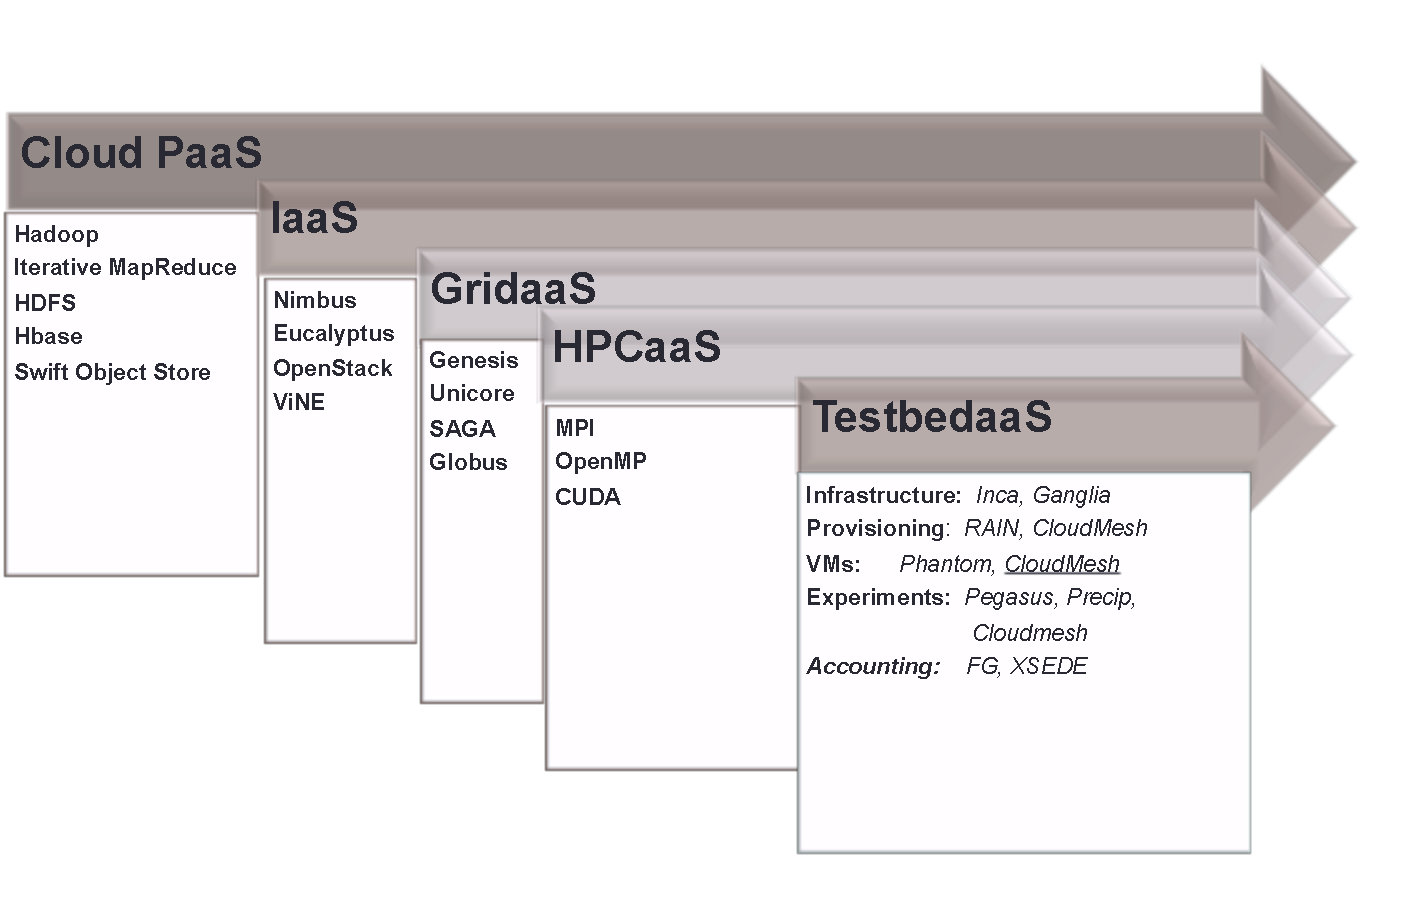
\includegraphics[width=0.9\textwidth]{images/user-services.pdf}
  \caption{FutureGrid high-level user services.}\label{F:services}
  ~\\
  \centering
  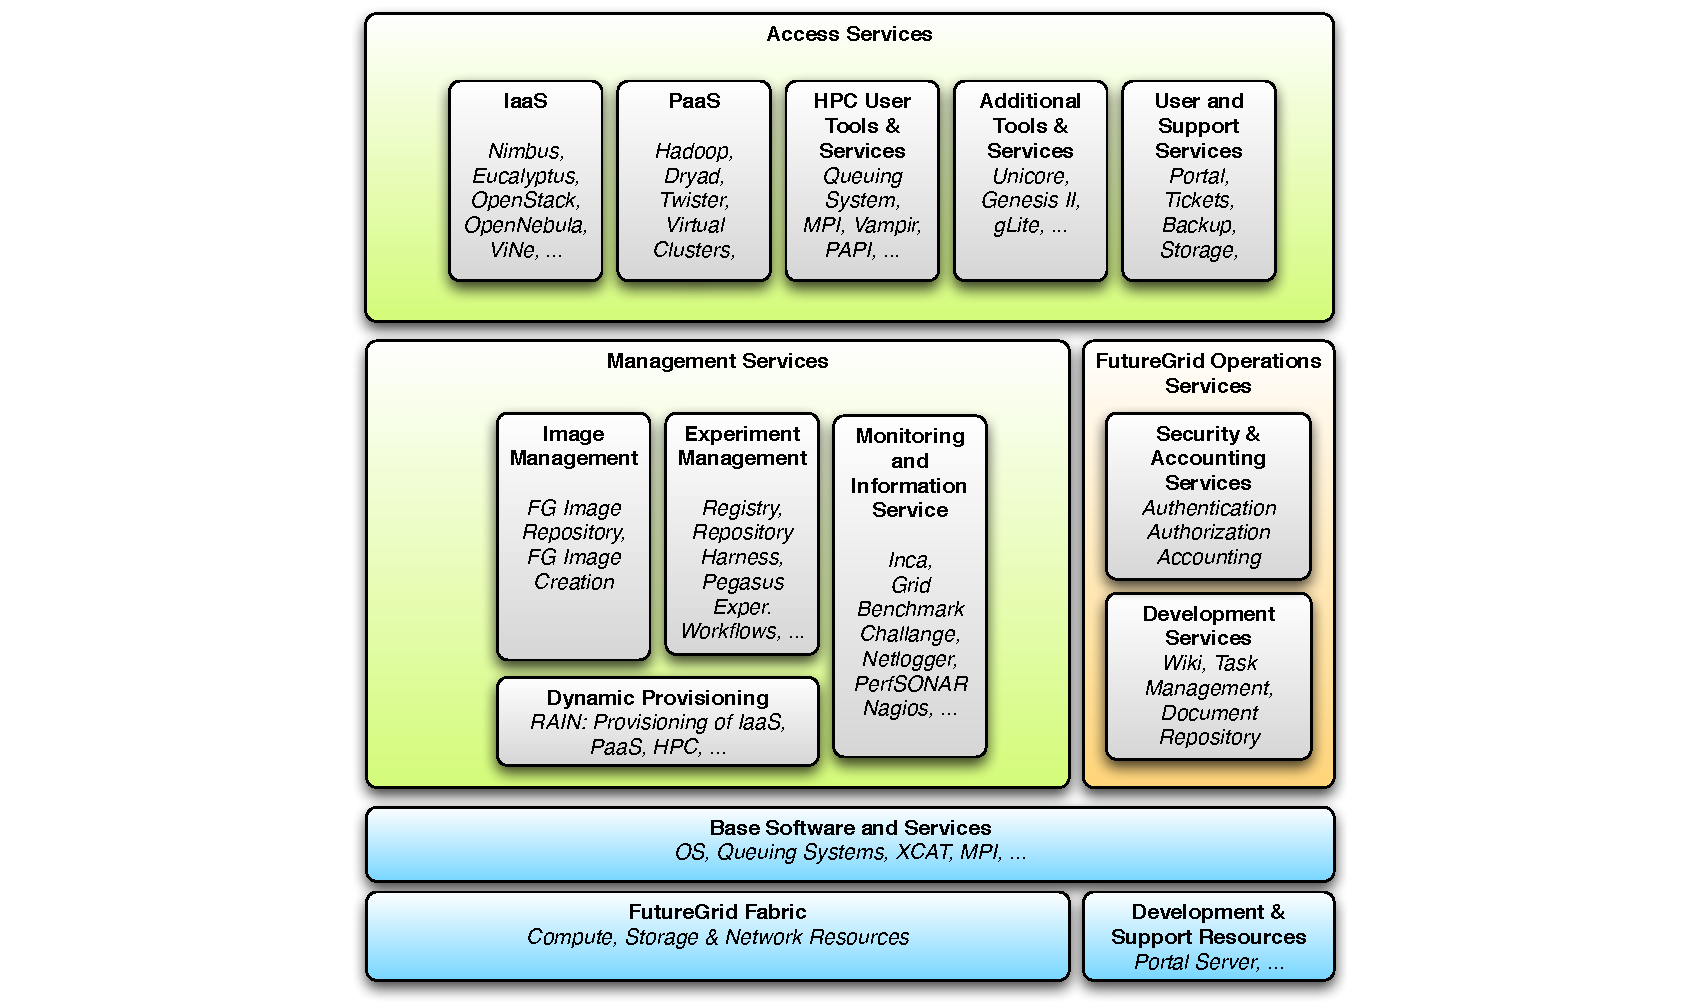
\includegraphics[width=0.9\textwidth]{images/architecture.pdf}
  \caption{FutureGrid high-level architecture.}\label{F:arch}.
\end{figure}

\subsection{Testbed as a Service (TestbedaaS)}

It is a well-accepted paradigm that today a lot of research including the one performed in big data is carried out by interdisciplinary scientific teams. Thus, FutureGrid provides an advanced framework to manage user and project affiliation and propagates this information to a variety of subsystems constituting the FG service infrastructure. This includes operational services (not explicitly mention in Figure \label{F:services}) to deal with authentication, authorization and accounting. In particular we have developed a unique metric framework that allows us to create usage reports from our entire Infrastructure as a Service frameworks. Repeatable experiments can be created with a number of tools including Pegasus, Precip and Cloudmesh. VMs can be managed on high level either via cloudmesh (see Section \ref{S:cloudmesh}). Provisioning of services and images can be conducted by RAIN \cite{imagemanagement,fg-1295}. Infrastructure monitoring is enabled via Nagios \cite{nagios}, Ganglia \cite{ganglia}, and Inca \cite{inca} and our own cloud metric system \cite{las08federated-cloud}.

\subsection{Traditional High Performance Computing as a Service (HPCaaS)}

Within the traditional high performance computing services FG offers a traditional MPI/batch queuing system and a virtual large memory system that are beneficial for big data calculations.

\subsubsection{MPI and Batch Queues}

The traditional high performance computing environment provided by queuing systems and Message Passing Interface (MPI) programs provide a suitable infrastructure not only for simulations, but also for the analysis of large data. However, considerable amount of work has to be conducted to optimize the available infrastructure to deal with distributed domain decompositions. Optimized use via traditional HPC has been successfully demonstrated for many biological applications. Additionally the existence of a queuing system can provide some advantages when the available resources are utilized to a full extend and resource starvation exists while sharing the resources with other users. This has been especially useful to support educational activities for classes with many users that for example want to test map reduce activities controlled by a queuing system as described in Section \ref{S:hadoop}.

\subsubsection{Virtual Large-Memory System}

One of the demands often posed in big data analysis it to place the data as much as possible into memory to speed up calculations and in some cases to fit the entire dataset into memory. However, this analysis may come at a cost as for example the use of HPC computing via MPI adds additional programming complexity within a cluster. Therefore it is desirable to virtualize the memory from multiple servers in a cluster to provide one big memory system that can be easily accessed by the underlying software.  One such implementation, vSMP by ScaleMP \cite{www-scalemp} \cite{las12fg-bookchapter}. vSMP is installed on the FutureGrid echo cluster that has 16 servers and can access up to 3TB in shared virtual memory.

\subsection{Grid as a Service (GridaaS)}

Not surprisingly the demand for computational Grids on FutureGrid has been relatively small. While we saw few requests for Globus we decided to focus on the installation of more popular systems. The little use can be explained by the availability of large Grid production infrastructure elsewhere such as in XSEDE and based on the move of the community away from complex Grid solutions to either cloud computing or even back to more traditional batch processing solutions. Furthermore, toolkits such as the CoG Kit also known as jglobus \cite{las05workflow-jgc,las01cog-concurency,las06-workflow-book} have provided enough abstractions for users that experimenting with such technologies has become less prominent and can be made on the client side while interfacing to production Grid services instead of testbeds. 

\subsection{Infrastructure as a Service (IaaS)}

One of the main features of FutureGrid is to offer its users a variety of infrastructure as a service frameworks \cite{comparisoncloud,las2011virt}. These frameworks provide virtualized resources to the users on top of existing cyberinfrastructure fabric. This includes but is not limited to virtualized servers, storage, network, disk, and other IaaS related services. In FutureGrid the most common hypervisor that runs the virtual machines as guest on the underlying operating system is KVM. Some resources also run XEN, however most recently the demand for KVM has increased and some services witll be switched from XEN to KVM. Through the ability to provide large numbers of virtual machines to the users, the access mode to utilize resources, in contrast to traditional HPC, has been changed from a reservation-based service to an on-demand service. This comes with the benefit that if enough resources are available they will be immediately allocated to the user. However if not enough resources can be offered the system will define the request and return with an error. Based on our experience with FG over the last couple of years it is advantageous to offer a mixed operation model. This includes a standard production cloud that operates on-demand, but also a set of reserved cloud instances that can be reserved for a particular project. We have conducted this for several projects in FutureGrid including those that required dedicated access to resources as part of big data research such as classes \cite{fg405,fg368} or research projects with extremely large virtual machines \cite{fg298}.

The IaaS services that are offered in FutureGrid contain the following:

\begin{description}
\item [OpenStack] has become most recently, next to HPC, the most requested services in FG based on newly started projects. OpenStack is an open source cloud infrastructure as a service framework to deliver public and private clouds. It contains a number of components that together build a powerful and flexible set to create a cloud service offering. Services include a compute service, and object storage, an image service, a monitoring service, and an orchestration service. OpenStack has received considerable momentum due to its openness and the support of companies. Within FutureGrid OpenStack clouds are currently deployed on India, Sierra, Hotel, and Alamo, while currently India provides the most up to date services.  

\item [Nimbus] is an open source service package allowing users to run virtual machines on FutureGrid hardware. Just as in Openstack users can upload their own virtual machine images or customize existing once. Nimbus, next to Eucalyptus is one of the earlier frameworks that make managing virtual machines possible. Nimbus provides a basic set of cloud services including services to easier orchestrate a cloud setup. However, Eucalyptus and OpenStack now also provide such services. 

Nimbus provides a selected subset of AWS protocols such as EC2. Accounting of Nimbus VMs does not provide currently features for project management. Such group-based and role based user management is essential for proper administrative resource and project management and is provided by other IaaS frameworks. In Nimbus it is  only conducted on a user-by-user basis. This has significant implications on user management as in large-scale deployments project management features are highly desired but are not offered in Nimbus. Although, a single users may not be interested in this feature, it is essential to provide proper project management of groups of users. 

\item [Eucalyptus] is an open source software IaaS framework for cloud computing. Eucalyptus provides an Amazon Web Services (AWS) compliant EC2-based web service interface to its users enabling the easy integration between a local cloud managed with Eucalyptus and AWS. However, as other IaaS frameworks such as OpenStack also provide EC2 interfaces for many application users OpenStack has become a viable alternative.

\end{description}

Which of the IaaS frameworks to chose is a question that is not that easy to answer. Many of our projects evaluate multiple of them to chose the one best suited for their use case. At other times users chose a framework that they have previously successfully used. Over time the quality of the IaaS framework has significantly changed. Within the last year OpenStack has become the most popular platform on FutureGrid.


\subsection{Cloud Platform as a Service (PaaS)}

\FILE{hadoop.tex}

\subsubsection{Map Reduce}

Map reduce models have been familiar to the programming and distributed computing community for a long time and have been historically associated with the functional programming's map and reduce. However the map and reduce framework introduced recently \cite{Dean:mapreduce} distinguishes itself from such efforts while applying it repeatedly, with fault tolerance on a very large distributed data set \cite{mapreduce-wikipedia}.

Instead of bringing the data to the computer in map reduce application we often use the concept of bringing the computing to the data. This makes a lot of sense when we assume that a large number of data is distributed over many servers and repeated search queries are cast to find results across them (as in the case of Google motivating map/reduce).

In general we can define a {\em map} step, that takes the input problem and divides it into smaller sub-problems distributing it among worker nodes. The map function is than executed on the data distributed on the various servers. The {\em reduce} step collects the answers of the subproblem and combines them in some fashion.

\begin{figure}[htb]
  \centering
    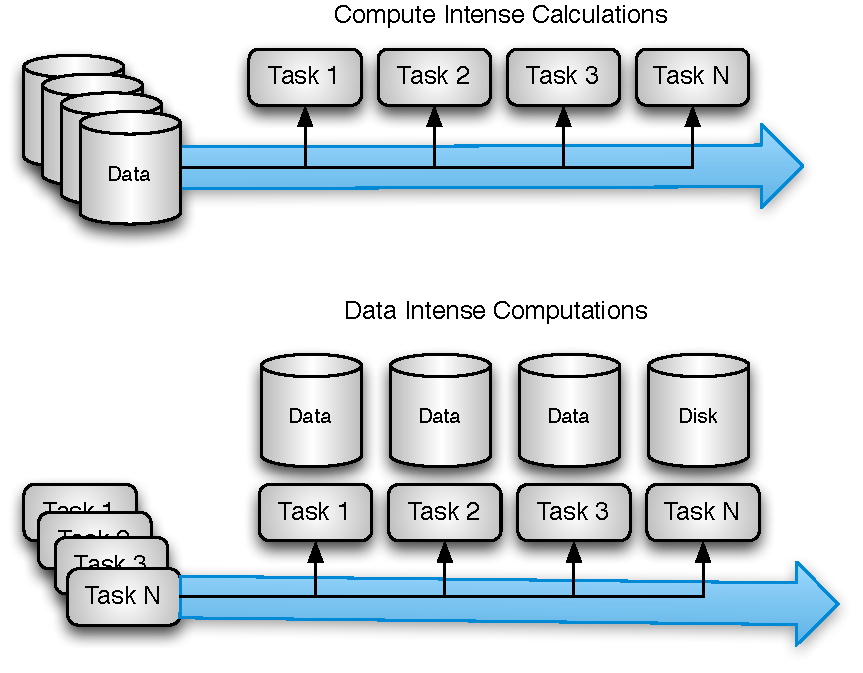
\includegraphics[width=0.75\textwidth]{images/mapreduce.pdf}
  \caption{Bring the data to the computation vs. bring the computation to tha data.}
\end{figure}

\paragraph{Hadoop.}\label{S:hadoop}

Hadoop \cite{www/hadoop} is an Apache project delivering an opensource software that uses the map/reduce framework in a distributed environment while focussing on scalability and reliability. Its design includes the Hadoop File System (HDFS) providing an easy to use file system to distribute the data among the servers on which the calculations will be executed. Hadoop is designed to deal with faults through redundancy which is an important feature when conducting data analysis on very large distributed databases \cite{www/hadoop}.  Hadoop is written in Java and provides the essential map reduce functionality and allows the system to be configured for existing hardware.

\paragraph{myHadoop.}

MyHadoop \cite{report/myhadoop}\cite{myhadoop2}, which is installed on many of the compute clusters in FutureGrid, enables to launch Hadoop clusters via traditional high-performance compute clusters. For this it utilizes the underlying batch scheduling system.

The reason for managing Hadoop jobs via a batch system may be multiple. First, the available infrastructure is resource constrained and utilization of disks and compute resources must be specially accounted for to allow shared usage by many users. This naturally happens in the educational research community quite frequently.  Second, to efficiently utilize the compute and data infrastructure researchers may not run Hadoop or MPI jobs continuously. At times they may need a Hadoop environment at other time they prefer a traditional message passing environment while at the same time being under resource constraints.

The idea of myHadoop is to submit a job to the queuing system that sets up a Hadoop cluster for the length of the reservation and the researcher can than use it to conduct experiments either via predefined jobs or in interactive mode. This is achieved by first identifying a number of resources via the scheduler, followed by the deployment of the Hadoop software across the identified servers. The user will than be presented with information on how to access this newly provisioned Hadoop cluster. myHadoop in it's new version \cite{myhadoop2} is supported for Oracle Grid Engine (formerly known as Sun Grid Engine), PBS, and SLURM.

Once Hadoop has been initialized, it can be accessed through regular job scripts as shown in Figure~\ref{F:myhadoop-script}. This example script uses eight nodes. It is important to set the processor per node to 1 to assure the various Hadoop daemons are scheduled on different servers. The rest of the script is not depicted as it contains the actual details on setting up Hadoop via the script and is beyond the scope of this chapter. The user should replace the text in $<...>$ to customize the job. As Hadoop is a user level program, it is also possible to run a user modified version of Hadoop which helps in adding new features or trying out newer versions of Hadoop than the default version that is installed for my Hadoop. The FutureGrid manual provides more details on how to practically use myHadoop on FutureGrid \cite{fg-manual-hadoop}.

\begin{figure}[htb]
\begin{center}
\begin{verbatim}
#!/bin/bash
#PBS -q <queue_name>
#PBS -N <job_name>
#PBS -l nodes=8:ppn=1
#PBS -o <output file>
#PBS -e <error_file>
#PBS -A <allocation>
#PBS -V
#PBS -M <user email>
#PBS -m abe

... details omitted
\end{verbatim}
\end{center}
\caption{PBS script to start hadoop}\label{F:myhadoop-script}
\end{figure}

\paragraph{Twister.}

Twister \cite{twsiter} is an extension to MapReduce to allow more easily the introduction of iterative map reduce processes. In addition twister has introduced a number of concepts including distinction between static and variable data, long running tasks, publish/subscriber based communication, and various other enhancements.  Twister is developed at Indiana University, and is used as part of classes on distributed systems and other educational activities. Hence it reaches popularity within FutureGrid.

\paragraph{Virtual Clusters.} In addition to the map/reduce platforms offered on FutureGrid, it is also possible to deploy virtual clusters. One of the earliest such framework has been showcased by von Laszewski \cite{github-futuregrid-vc} while deploying a SLURM cluster. Such a cluster can than be used as a teaching tool or provides additional mechanisms to custom create queues and reservations. However, the most advanced feature of FutureGrid will be via cloudmesh, which will allow the deployment of clusters not only in virtual machines, but on bare metal.


\FILE{usage.tex}

\section{FutureGrid Usage}\label{S:usage}

When offering services such as FutureGrid to the community, we have to analyze and predict which services may be useful for the users. We have therefore established a number of activities that monitor external and internal data. Externally, we look for example at information provided by Gartners technology hype curve \cite{www-gartner-2013} or Google trend information as shown in Figure \ref{F:google-trend}. From Google Trend data we observe that the popularity of Grid computing has been very low in the recent years and much attention has shifted to cloud computing. Therefore we removed this information from the figure and focus exemplary on cloud related terms such as {\em Cloud Computing}, {\em Big Data}, {\em OpenStack} {\em VMWare}.  From this information we see that all but VMWare are rising, with Cloud Computing dominating the Google trends in comparison to the others. This trend is important as it shows a shift in the cloud computing community buzz away from a traditional commercial market leader in virtualization technology. We believe that is correlated with a large number of vendors offering alternative products and services while at the same time the novelty from VMWare is reduced.

\begin{figure}[htb]
 \centering
    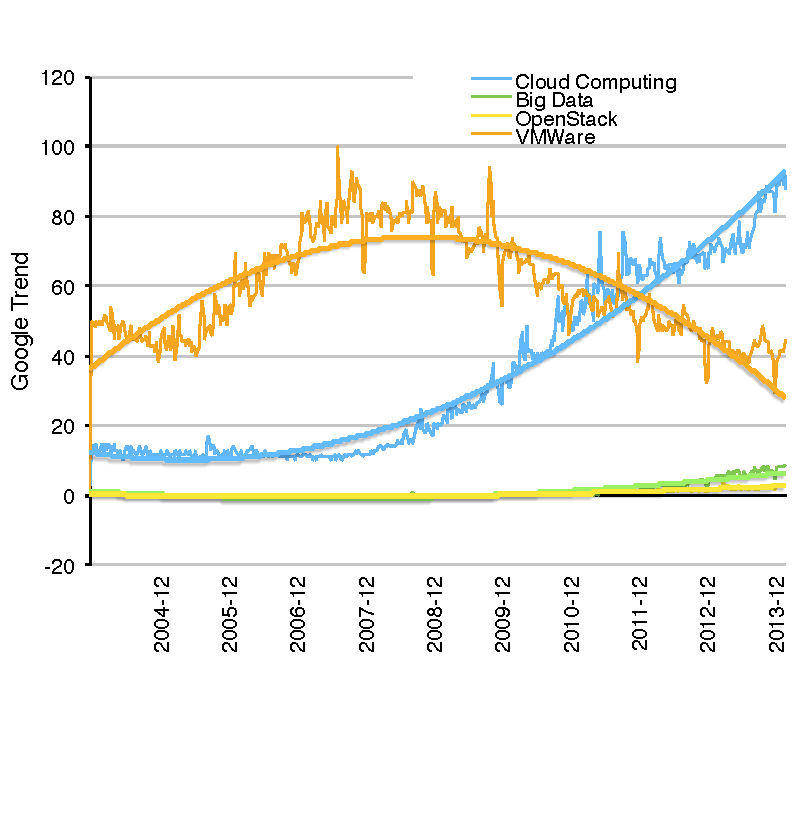
\includegraphics[width=.75\textwidth]{images/google-trend.pdf}
  \caption{Google Trends.}\label{F:google-trend}
\end{figure}

To give an informal overview of the more than 300 projects conducted on FutureGrid we have taken their titles and display them in a word cloud (see Figure \ref{F:wordcloud}. Additionally, we have taken keywords that are provided by the project leads and also displayed the in a word cloud (see Figure \ref{F:keycloud}. Although the images doe not give quantitative perspective about the project it helps to identify some rough idea about the activities that are ongoing in FutureGrid.  As expected the terms cloud computing an and terms such as mapreduce, OpenStack, Nimbus, and Eucalyptus appear quite frequently. It is hence worthwhile to analyze this data in a more quantitative form.

\begin{figure}[p]
\begin{minipage}[t]{1.0\textwidth}
  \centering
    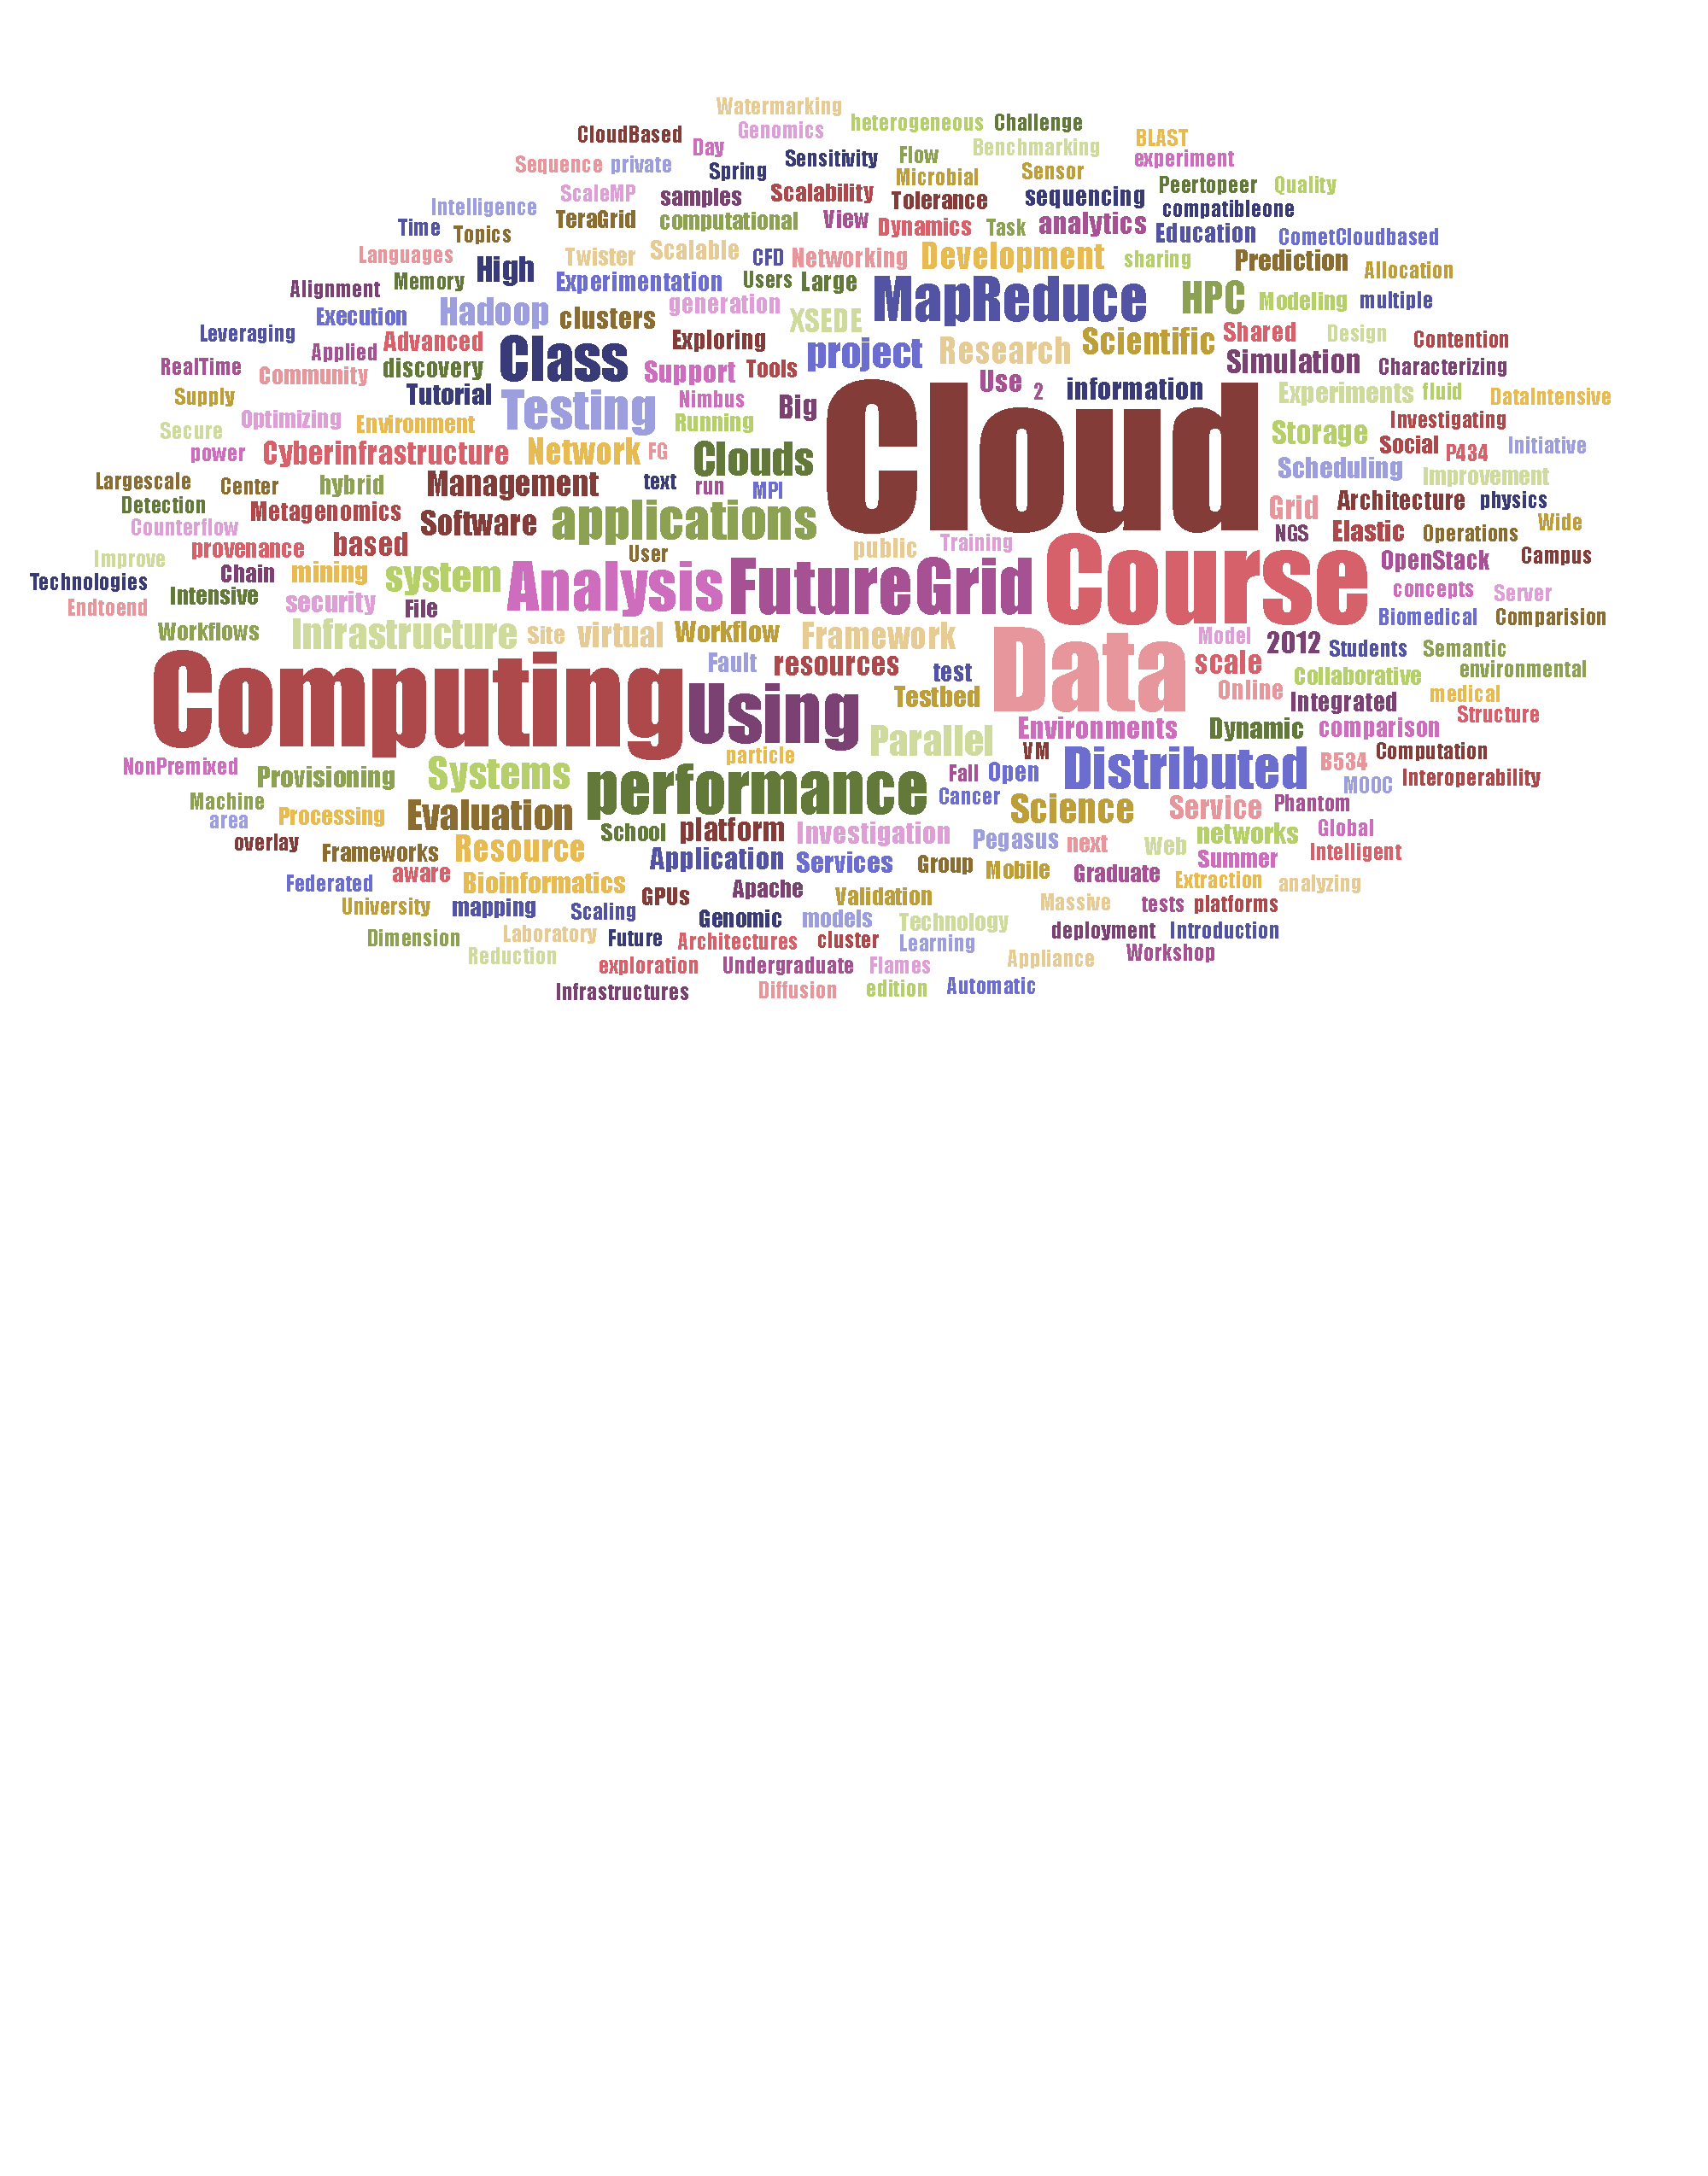
\includegraphics[width=1.0\textwidth]{images/fg-title-wordcloud.pdf}
  \caption{Project title word cloud.}\label{F:wordcloud}
\end{minipage}
\vspace{24pt}\\
\begin{minipage}[t]{1.0\textwidth}
  \centering
    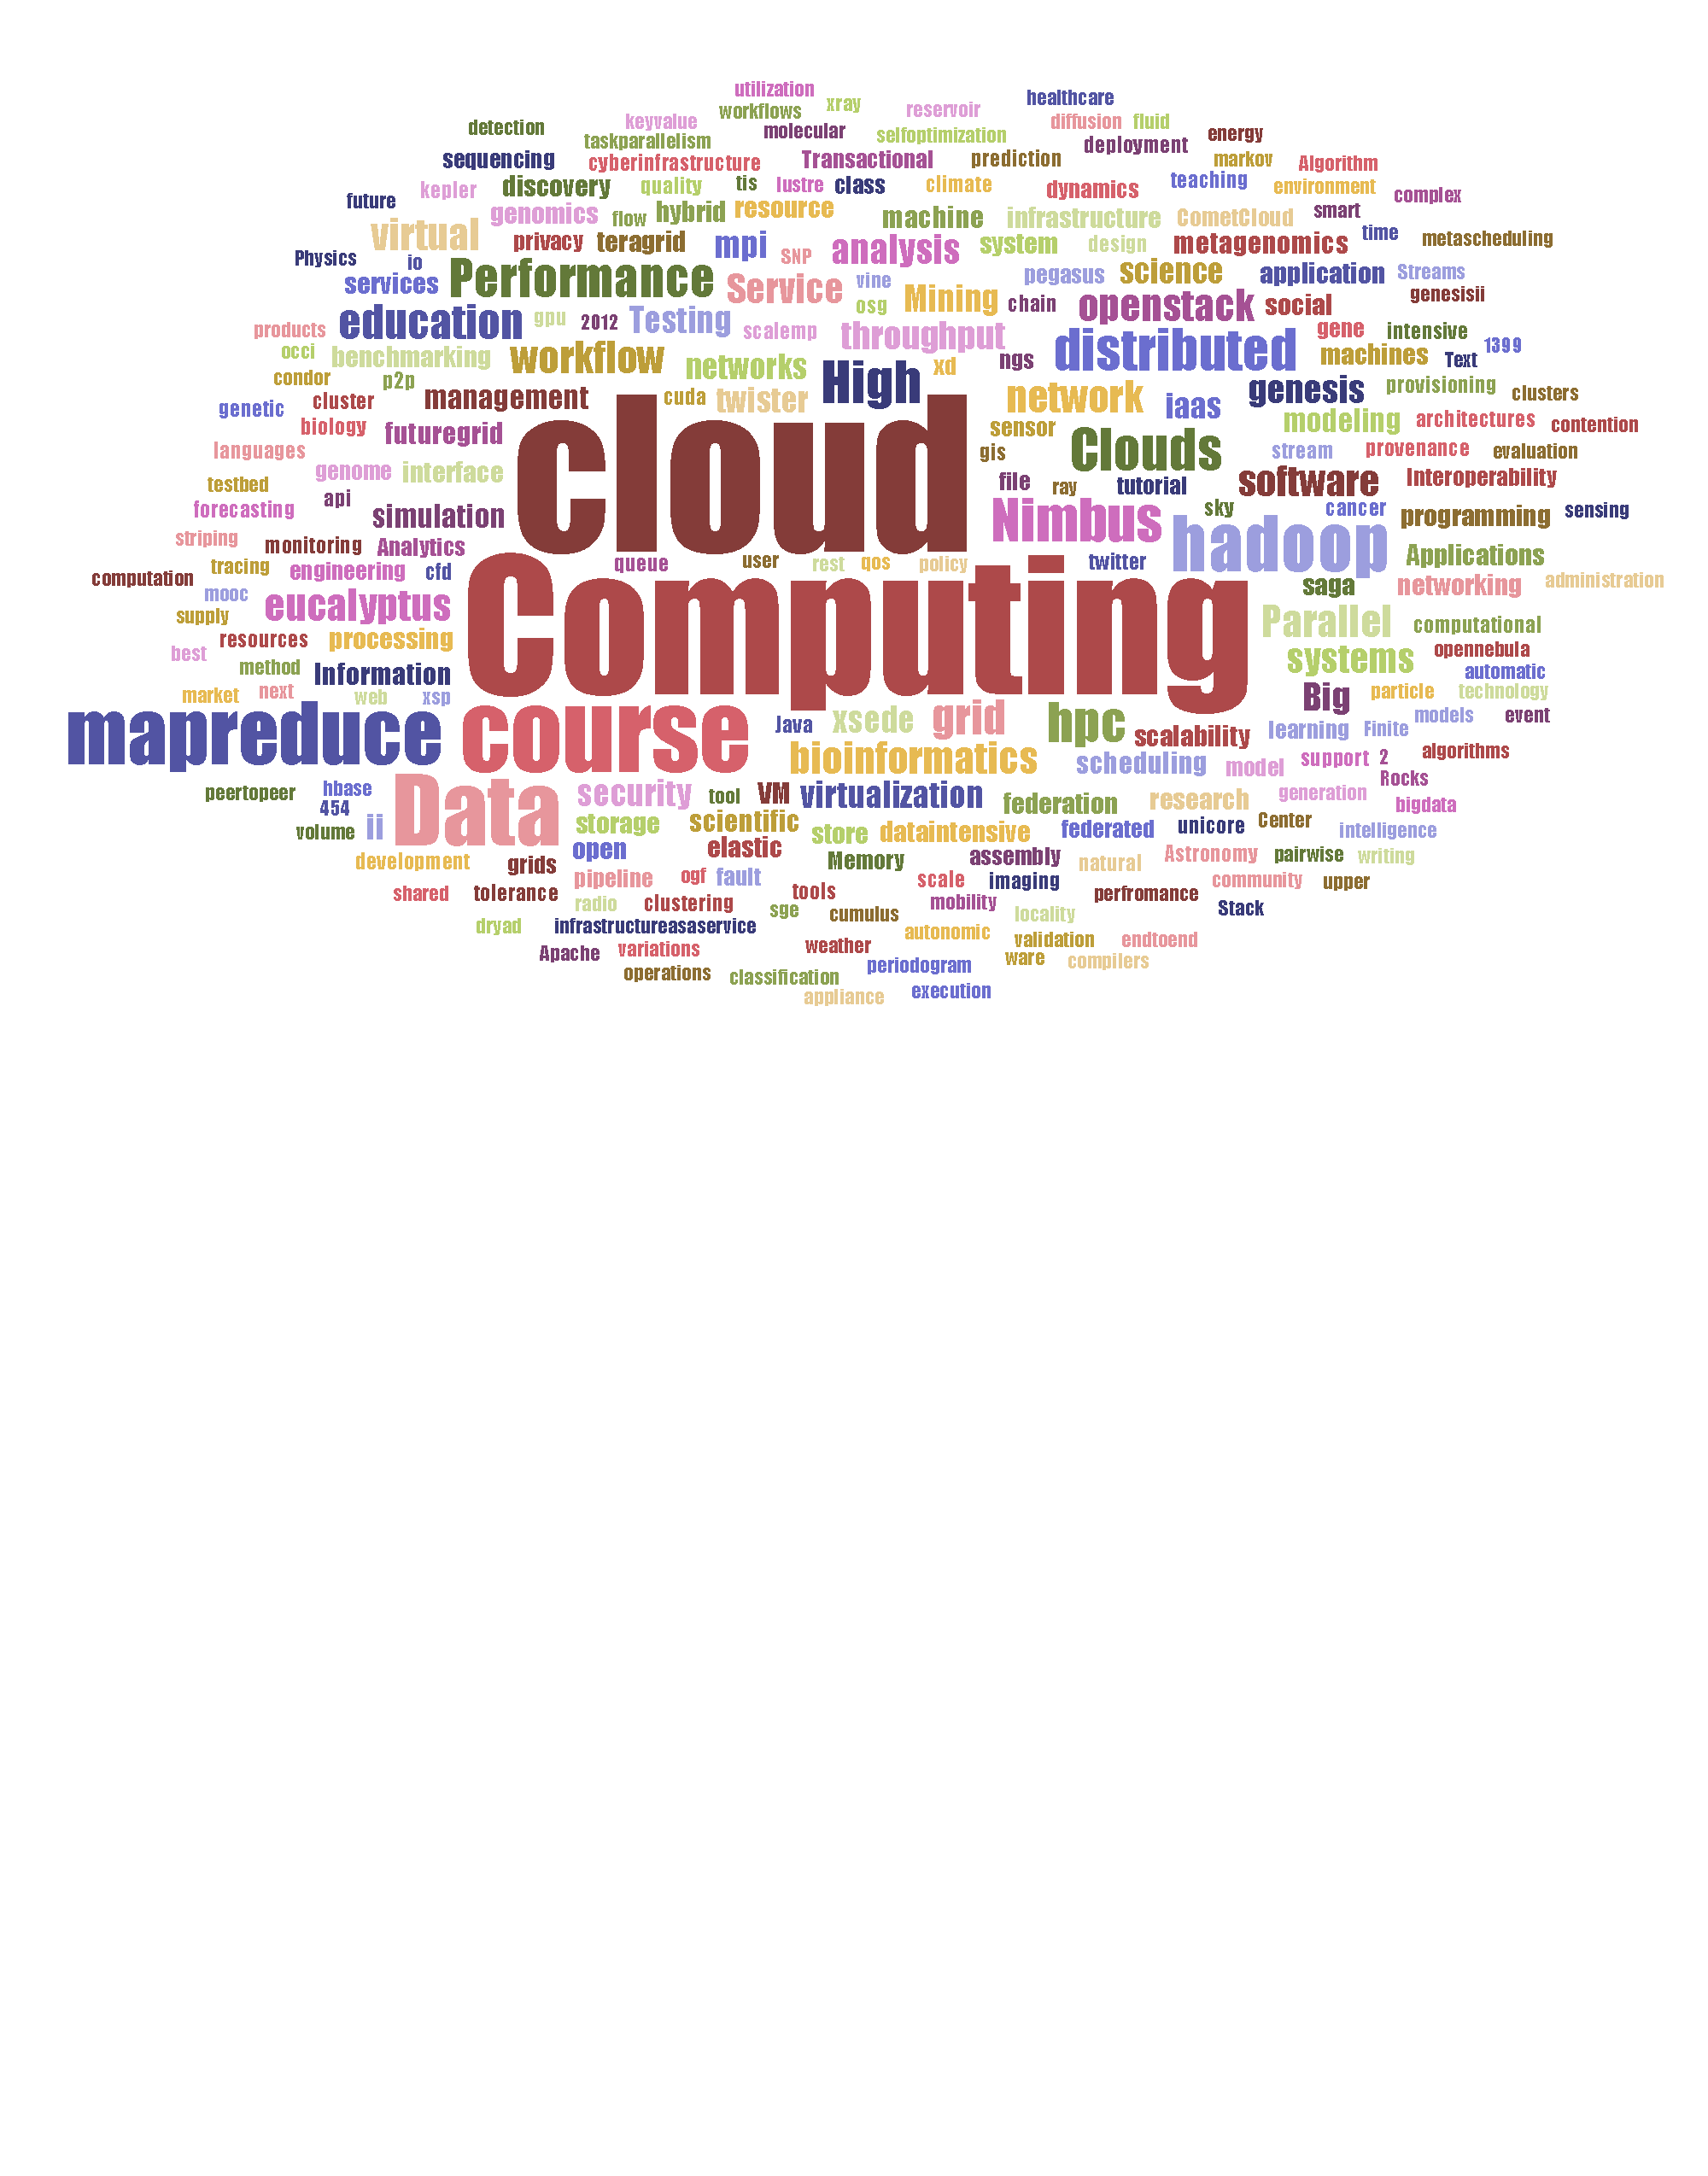
\includegraphics[width=1.0\textwidth]{images/fg-keyword-wordcloud.pdf}
  \caption{Project keyword word cloud.}\label{F:keycloud}
\end{minipage}
\end{figure}


As part of our project management in FutureGrid we have designed a simple project application procedure that includes prior to a project granted access gathering information about which technologies are anticipated to be used within the project. The list is fairly extensive and includes Grid, HPC, and Cloud computing systems, services, and software. However, for this paper we will focus primarily on technologies that are dominantly requested and depicted in Figure~\ref{F:request-tech}. Clearly we can identify the trend, that shows the increased popularity of OpenStack within the services offered on FutureGrid. Nimbus and Eucalyptus are on a significant downwards trend. ObenNebula was also at one point more requested than either Nimbus or Eucalyptus, but due to limited manpower an official version of OpenNebula was not made available on FutureGrid. As we have not offered it and pointed it out on our Web page, requests for OpenNebula have vanished.  However internally have used OpenNebula for projects such as our cloudmesh rain framework. All other sixteen technologies are relatively equally distributed over the monitoring period. The lesson that we took form this is that FutureGrid has put more emphasize in offering OpenStack Services recently.

\begin{figure}[htb]
  \centering
    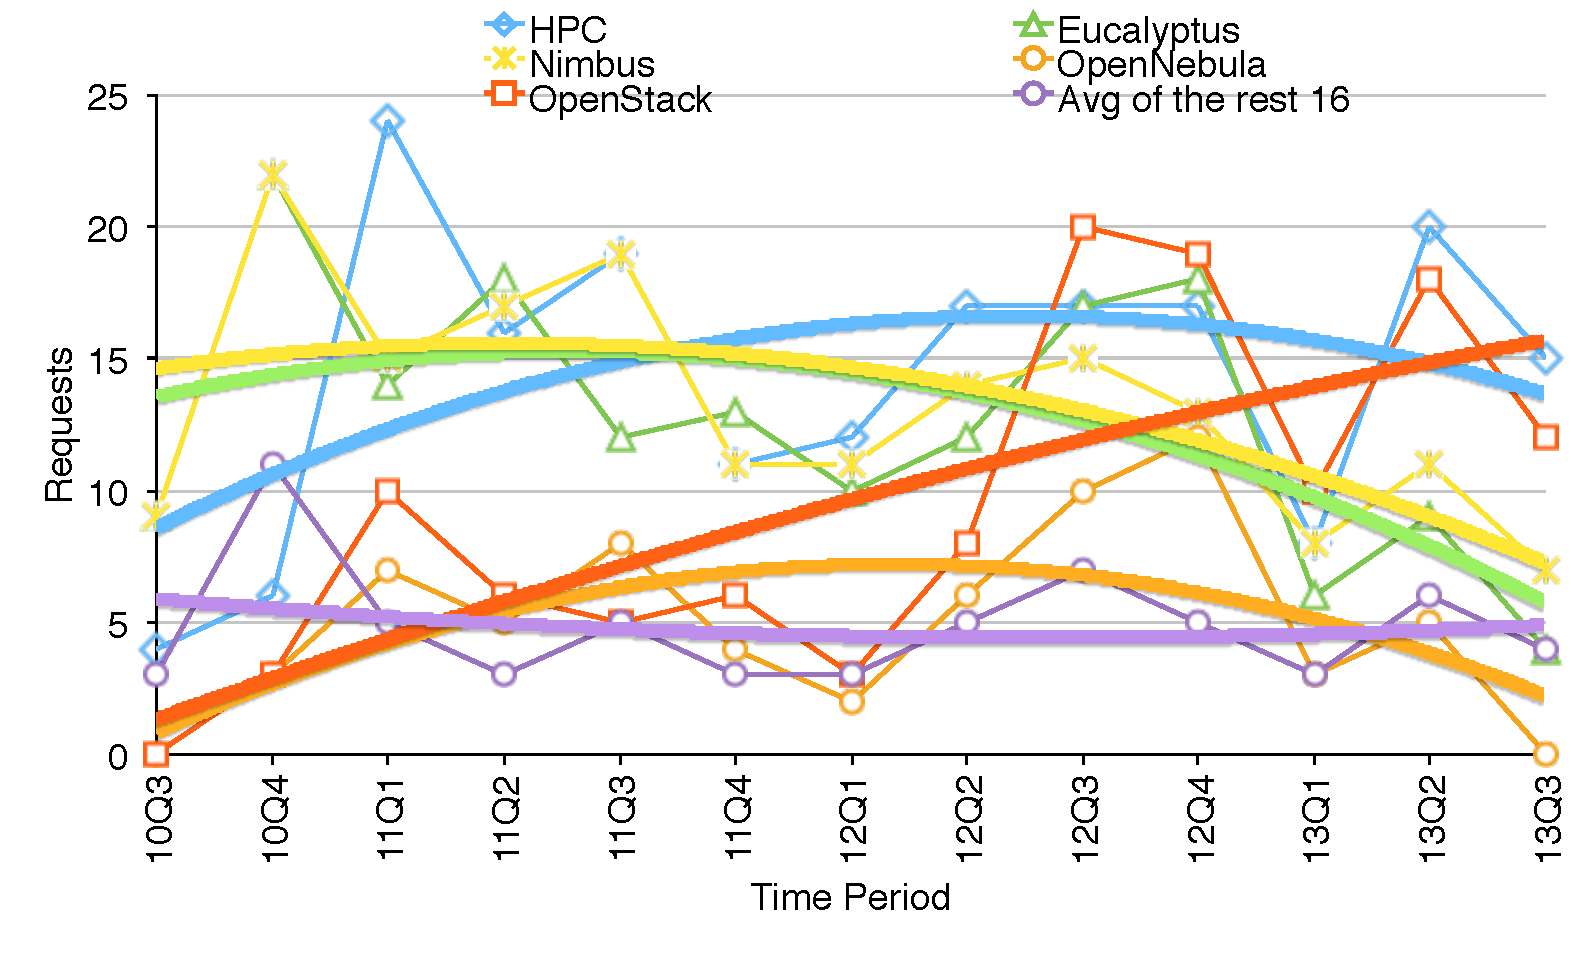
\includegraphics[width=1.0\textwidth]{images/trend-a.pdf}
  \caption{Requested technologies by project}\label{F:request-tech}
\end{figure}

\begin{figure}[p]
 \centering
    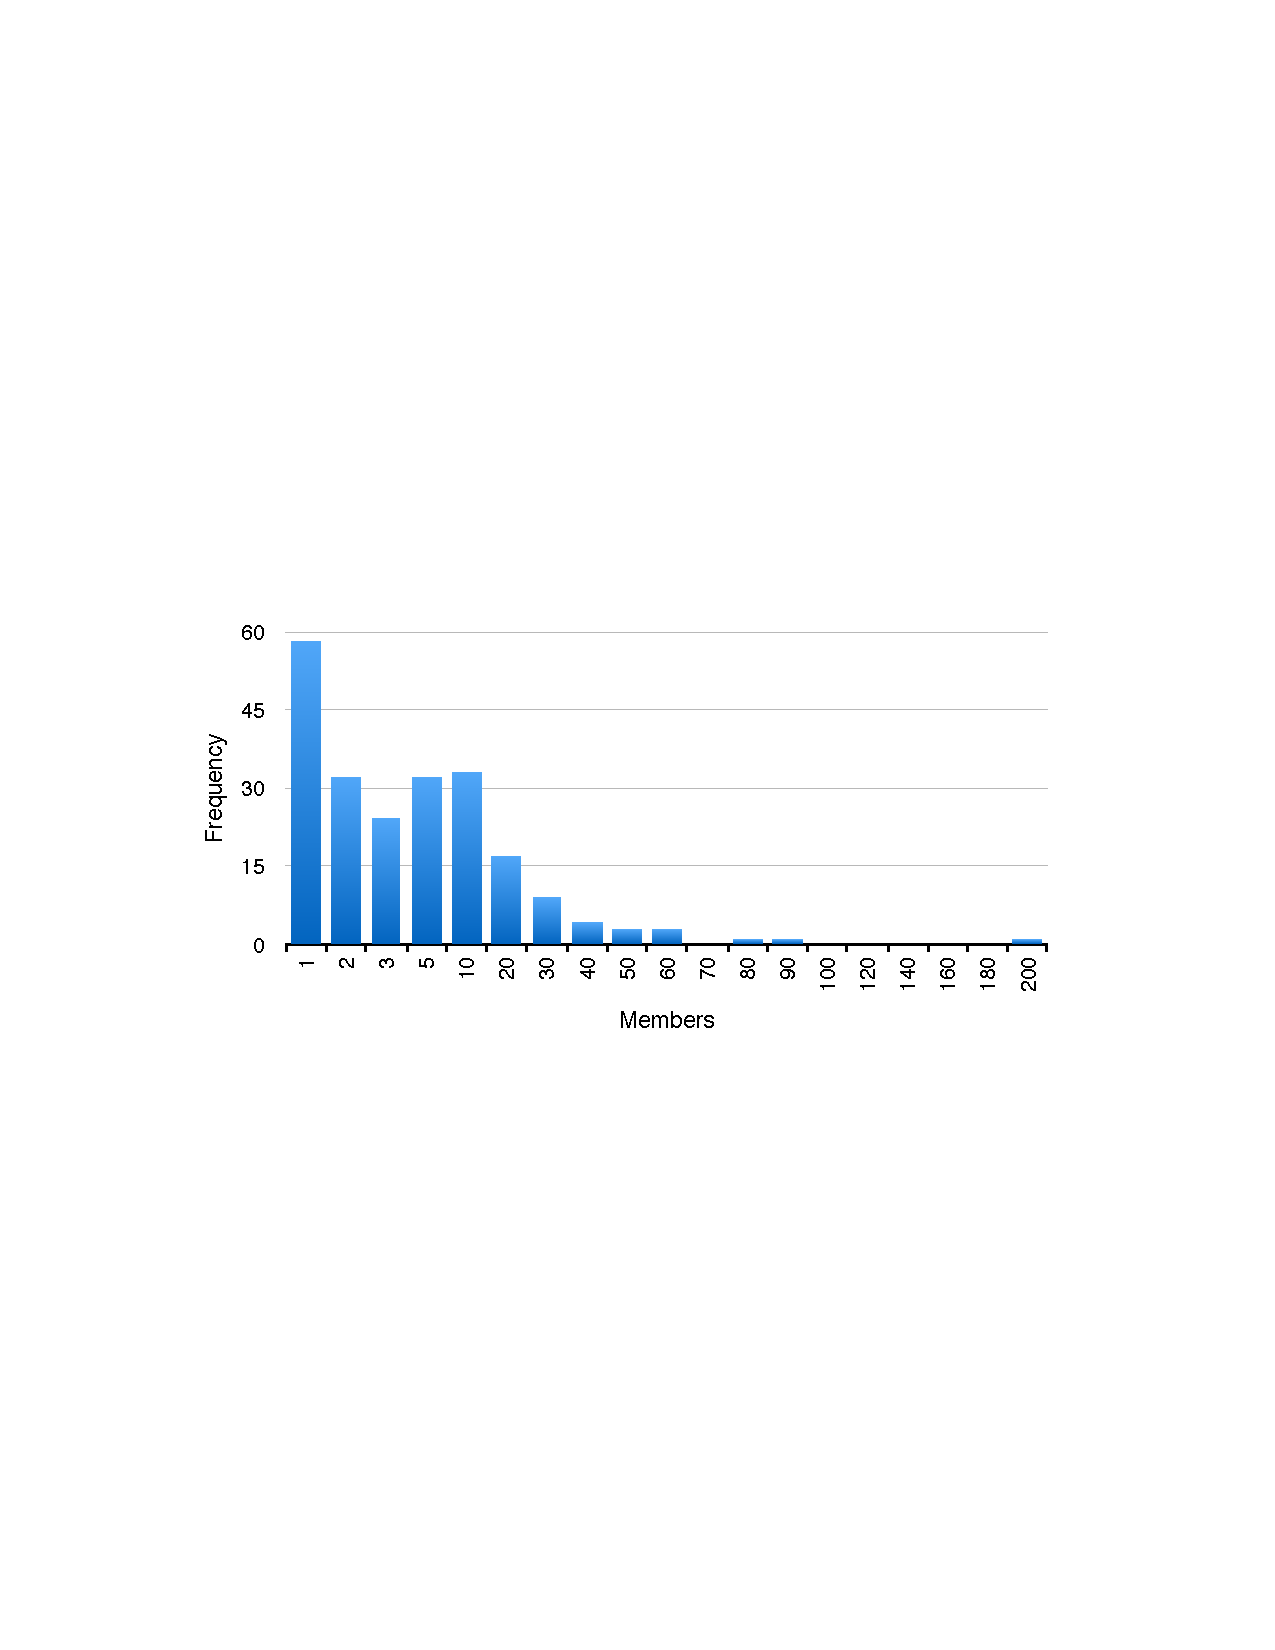
\includegraphics[width=.7\textwidth]{images/project-frequency.pdf}
  \caption{Project Frequency.}\label{F:project-members}

  \centering
    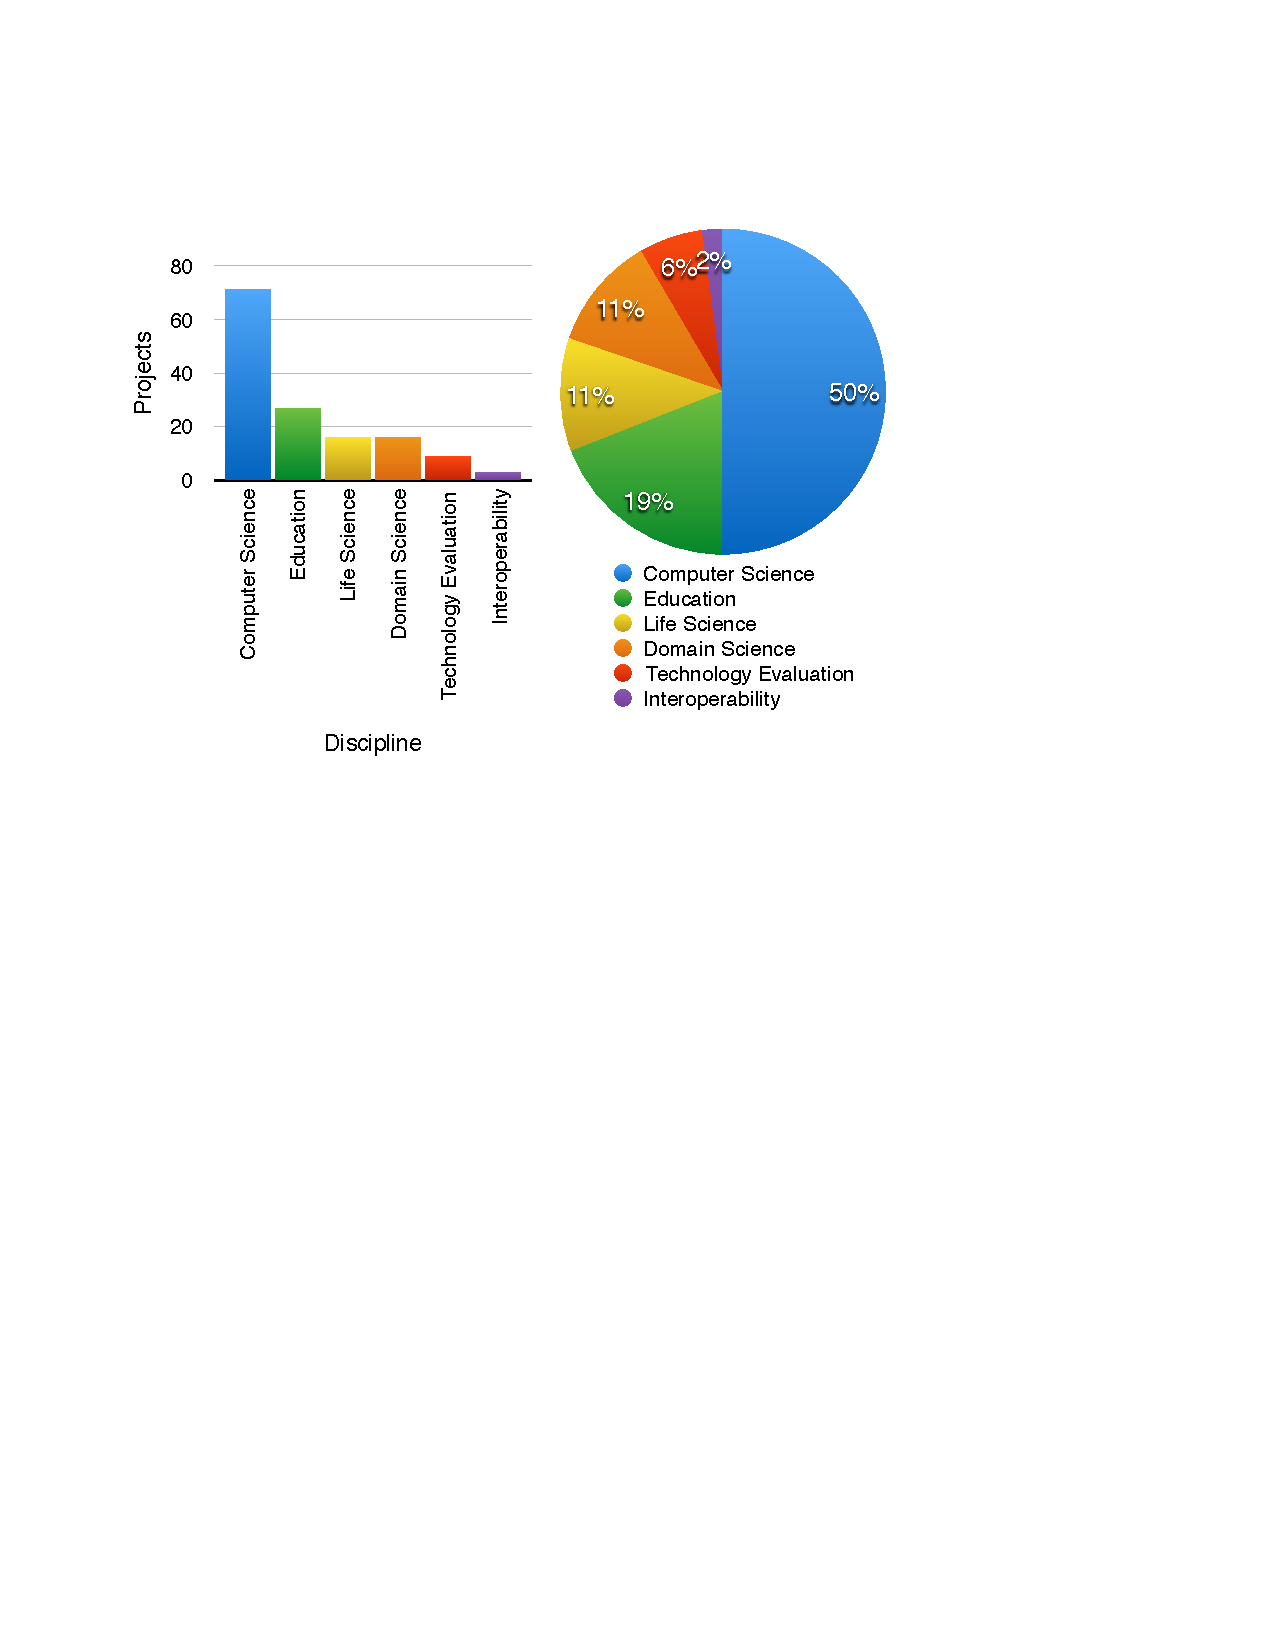
\includegraphics[width=.6\textwidth]{images/project-disciplines.pdf}
  \caption{Distributon of project disciplines.}
  \label{F:freq-dis}

  \centering
    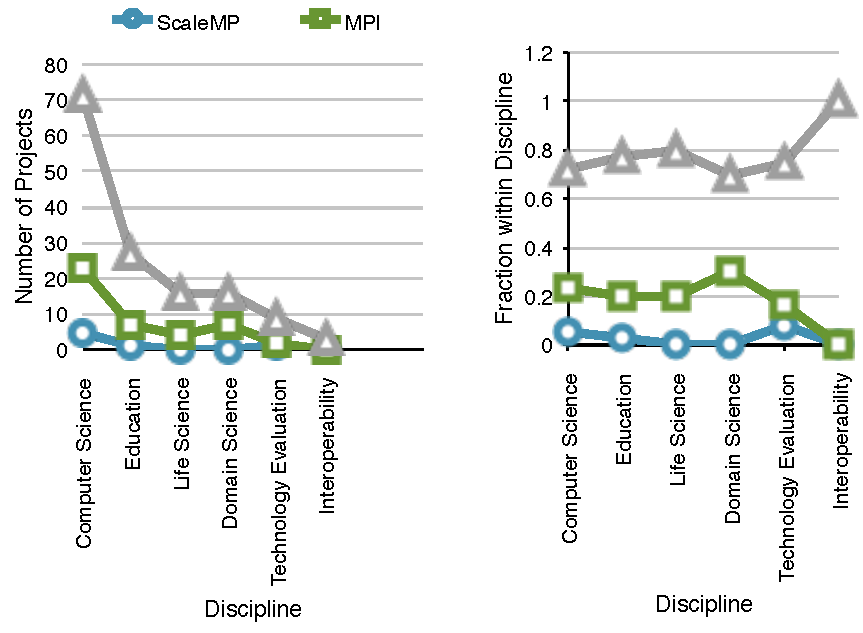
\includegraphics[width=.75\textwidth]{images/trend-b.pdf}
  \caption{Requests by of technologies by discipline within a
    project. $\bigtriangleup$ = Map Reduce, Hadoop, or Twister,
    $\Box$  = MPI, $\circ$ = ScaleMP}
   \label{F:trend-b}
\end{figure}

From the overall project information we have also analyzed the frequency of the number of project members within the project and show it in Figure~\ref{F:project-members}. Here we depict on the abscissa classes of projects with varying members.  Assume we look at the abscissa value of 10, This means that these are all projects that have project members between 10 and its previous category in this case 5. Hence, it will be all projects greater 5 and smaller or equal 10. With this classification we see that the dominant unique number of members within all projects is either one, two or there members. Than we have another class between 4 and 10 members, and the rest with more than ten members. One of the projects had overall 186 registered members, for an education class as part of a summer school. Looking at the distribution of the members and associating them with research and education projects, we find all projects with larger numbers of projects to be education projects.



%Figure~\ref{F:bigdata-freq} shows the frequency distribution of technologies such as
%map/reduce, hadoop, and twister by year. In the chart we simply called
%the agglomoration of these technologies big data.  As we see relative
%to all projects requested within one year we identified a rising trend.

%\begin{figure}[htb]
%  \centering
%    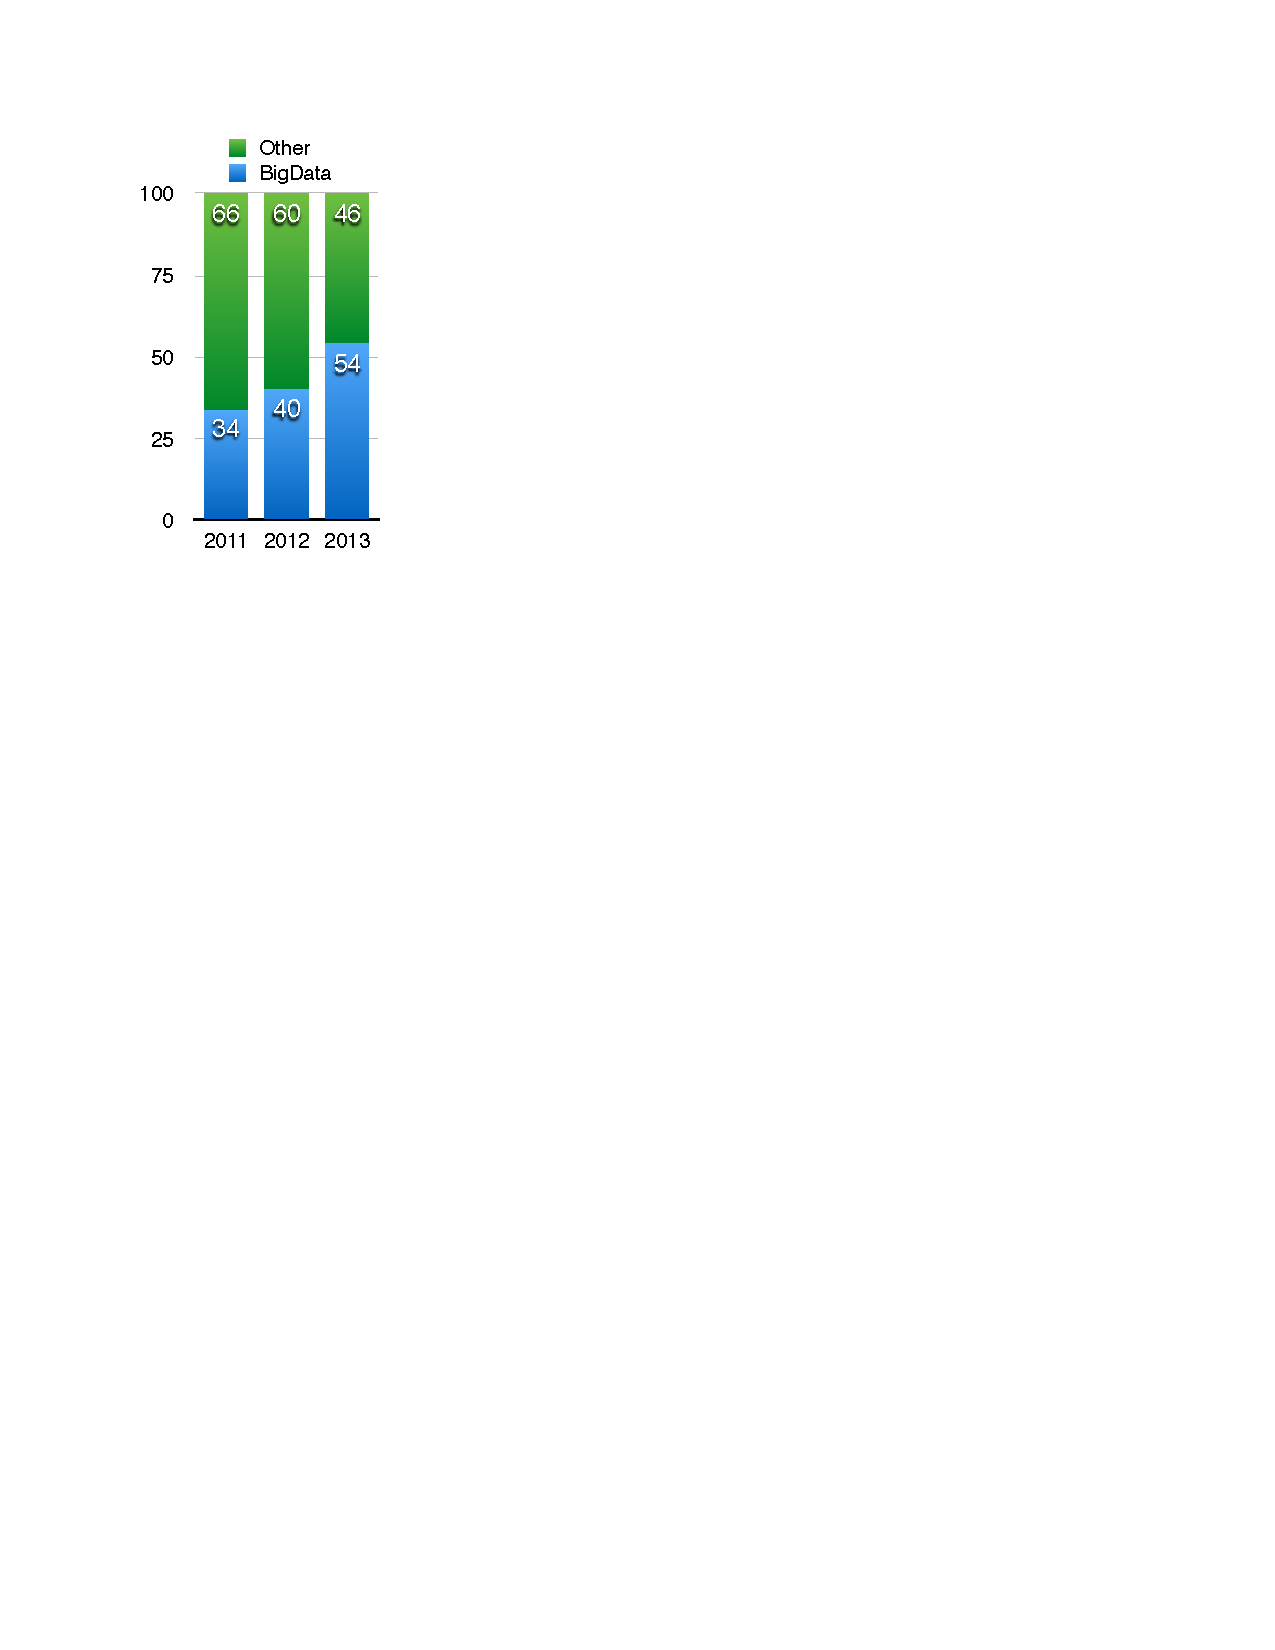
\includegraphics[width=0.2\textwidth]{images/bigdata-freq.pdf}
%  \caption{Big Data Project frequency.}\label{F:bigdata-freq}
%\end{figure}

Next we have analyzed all projects that requested either mapreduce, hadoop, twister, MPI and ScaleMP (147 of all 374 active projects, which is 39\% of all projects) and categorized them by discipline as shown in in \ref{F:freq-dis}. In contrast to XSEDE which provides a production HPC system to the scientific community, the usage of FutureGrid for map reduce  frameworks is dominated with 50\% by computer science related projects followed by education with 19\%.


If we look at further into this data we present in Figure \ref{F:trend-b} the number of projects in a particular category, as well as the Fraction of technologies within a discipline. As we are in this paper interested in the impact on big data. we have looked in particular at requests for mapreduce, Hadoop, and twister, awhile also looking at requests for MPI and ScaleMP. It is interesting to note that the percentual distribution of the technologies among these projects is about constant if we exclude technology evaluations and interoperability. As MPI is more popular with domain sciences we find a slight increase in projects requesting MPI. However with the life sciences we see the opposite as map/reduce and associated technologies are more popular here. MPI and ScaleMP are not much requested as part of technology evaluations and interoperability experimentation is as they either project a very stable framework and does not require evaluation, or the question of interoperability is not of concern for most of the projects.  




%\begin{figure}[htb]
%  \centering
%    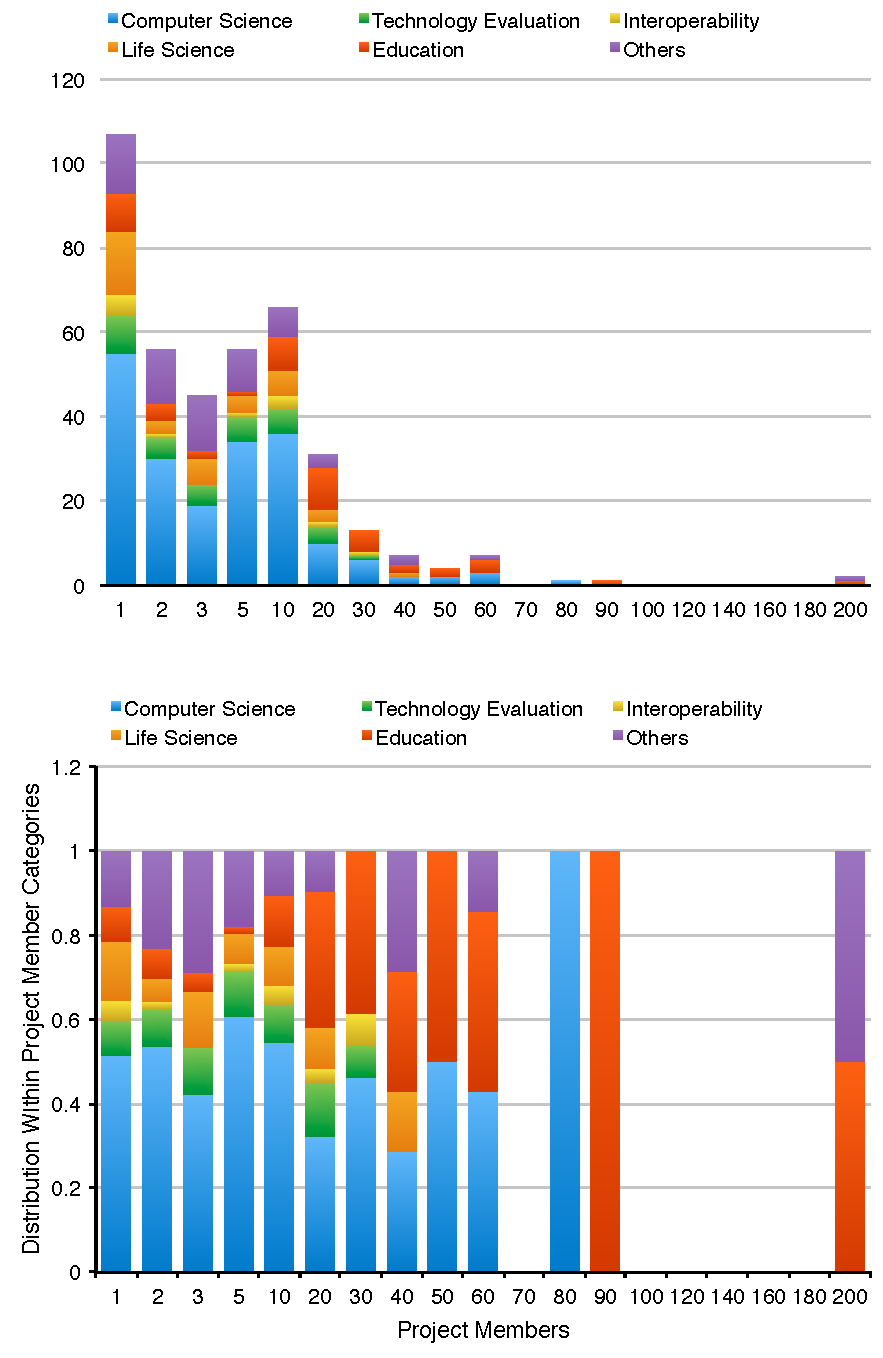
\includegraphics[width=1.0\textwidth]{images/project-member-dist.pdf}
%  \caption{Project Member Dist.}
%\end{figure}

%\afterpage{\clearpage}

\FILE{devops.tex}

\section{System Management}\label{S:devops}

The goals of FutureGrid to offer a variety of services as part of its testbed features is going beyond services that are normally offered by data and supercomputing centers for research. This provides a number of challenges that need to be overcome in order to efficiently manage the system and provide even services that have never been offered to users as they exist on FutureGrid.

\subsection{Integration of Systems and Development Team}

FutureGrid started initially with a model where the systems team and the software team were separated. An unnecessary wall between teams was erected that resulted in multiple challenges:

\begin{enumerate}

\item The system setup and management was  completeley separated from the software development team focusing mostly on the deployment of existing technologies. However the technologies deployed were themselfs under heavy development and require intercorrelations between developers and system teams.

\item The deployed system was complex, but its deployment was documented to a limited extend not allowing the developers to utilize it properly or knowing what has been deployed and utilize it properly.

\item Lack of trust by the systems team did not allow the software team to have a valid development environment as proper privileges were not issued to the developers. As the development teaam needed to use priovilkedged system services the development could not be carried out.

\item The software developed needed a testbed within the testbed that was not necessarily reflecting the actual system setup.

\end{enumerate}

Together these issues, made it extremely difficult if not impossible to further any development in regards to the design of a testbed infrastructure as requested by our original ambitious goals.

To overcome these difficulties it was decided early on in the project that the systems team must be integrated in some fashion into the software team and become part of the development process. This integration is not an isolated instance within FutureGrid, but is also executed in many modern data centers and is now recognized with its own term called {\em DevOps}.

\subsection{DevOps}

DevOps is not just a buzzword from industry and research communities, but it provides value added processes to the deployment and development cycles that are part of modern data centers. It can today be understood as a software development method that stresses collaboration and integration between software developers and information technology professionals such as a system administrator.

While using an infrastructure such as clouds we recognized early on that the lifetime of a particular IaaS framework is about 3-6 month before a new version is installed. This is a significant difference to a traditional High Performance Computing Center that is comprised of many software tools experiencing much longer life spans. This is not only based on security patches but significant changes for example in the evolving security infrastructure, user services as well as the deployment of new services that become available in rapid procession.

This rapid change of the complex infrastructure requires a rethinking about how systems in general are managed and how they can be made available to the development teams. While previously it may have been enough to install updates on the machines, DevOps frameworks provide the developer and system administrators to create and share environments that are used in production and development while at the same time increasing quality assurance by leveraging each others experiences (see Figure \ref{F:devops}).

\begin{figure}[htb]
  \centering
   \begin{minipage}{.5\textwidth}
    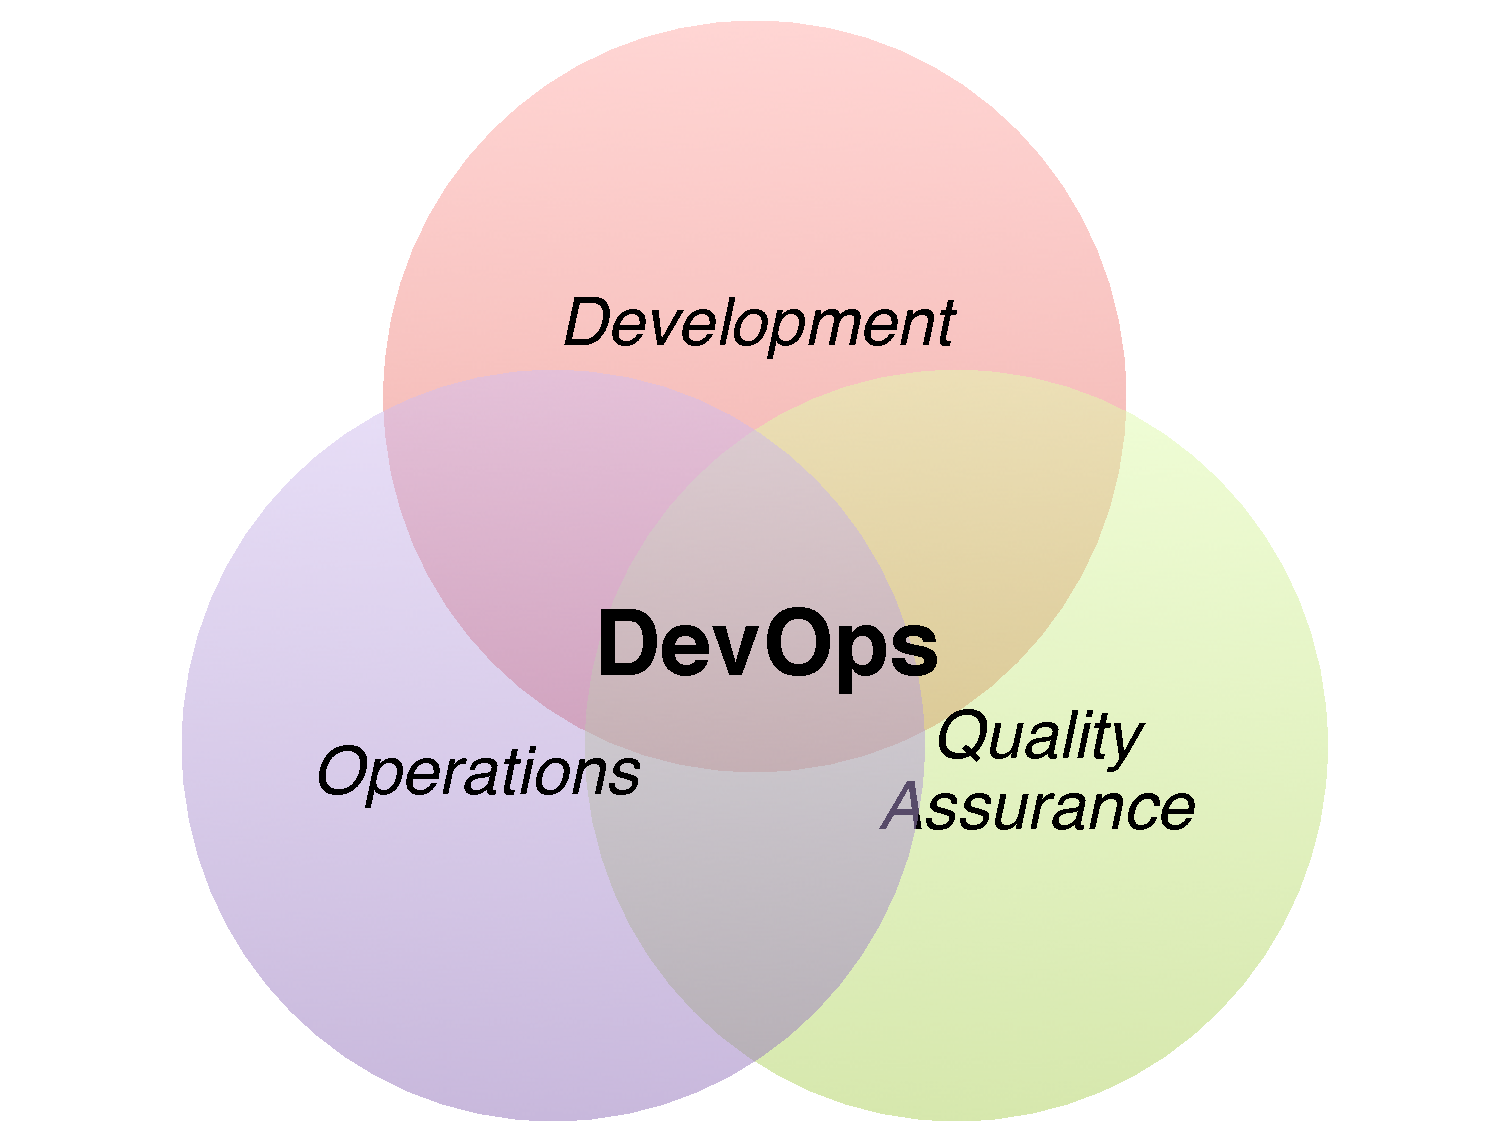
\includegraphics[width=1.0\textwidth]{images/devops.pdf}
    \caption{DevOps Intersection.}
    \label{F:devops}
  \end{minipage}%
   \begin{minipage}{.5\textwidth}
     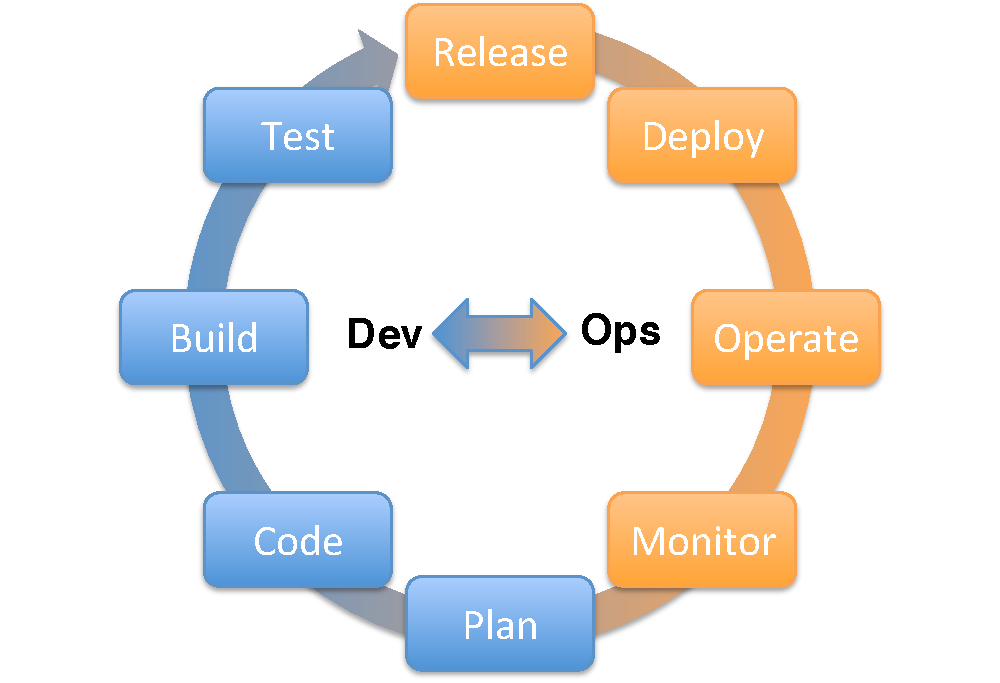
\includegraphics[width=1.0\textwidth]{images/devops-circle.pdf}
     \caption{DevOps Cycle.}
     \label{F:devops-circle}
  \end{minipage}%
\end{figure}

\paragraph{DevOps Cycle.}

While combining the steps executed by the development and operational team from planning, to coding, building and testing, to the release, deployment and operation and monitoring (see Figure \ref{F:devops-circle}), each of the phases provides a direct feedback between the DevOps team members and shortening thus the entire development phase. It also allows testing out new services and technologies in a rapid progression. Hence it is possible to roll out new developments much faster into production. This leads to a much more rapid integrated cycle than without the correlation between development and operation would be possible.

\paragraph{DevOps Supporting Tools.}

A number of tools are available that make the introduction of DevOps strategies more efficient. The first is the need for an efficient communication pathway to manage tasks not only between developers but also between users. Thus the ideal system would provide a complete integration of a project management system that allows managing tasks for both developers and operators, but also to easily integrate tickets and transform them into tasks. In XSEDE and other supercomputing centers a system called RT \cite{www-rt} is typically used for user ticket management. Other systems such as jira, mantis, and basecamp are often used to manage the software and systems related tasks. Unfortunately, personal or organizational constraints prevent often the integration of the two systems and additional overhead is needed to move user tickets into tasks and the development cycle. Within FutureGrid we experimented as part of our opensource development extensively with jira as systems and ticketing system \cite{www-jira-ticket} reveling that newest development in such areas motivated by DevOps teams lead to tools that support the overall cycle including user ticket management in a single system (see Figure \ref{F:usedevops}). However, the integration of FutureGrid within the overall much larger XSEDE effort did make it not possible to switch from RT to jira for user ticket management. To stress this user integration we term this framework {\em UseDevOps}. Tools to integrate Development and Operation deployment include puppet, chef, ansible, cfengine and bcfg2. While FutureGrid started out with bcfg2 we have since than switched to other tools due to their prevalence within the community. Chef, puppet, and ansible have significant amount of traction. Due to expertise within our group we currently explore chef and ansible.

\begin{figure}[htb]
  \centering
    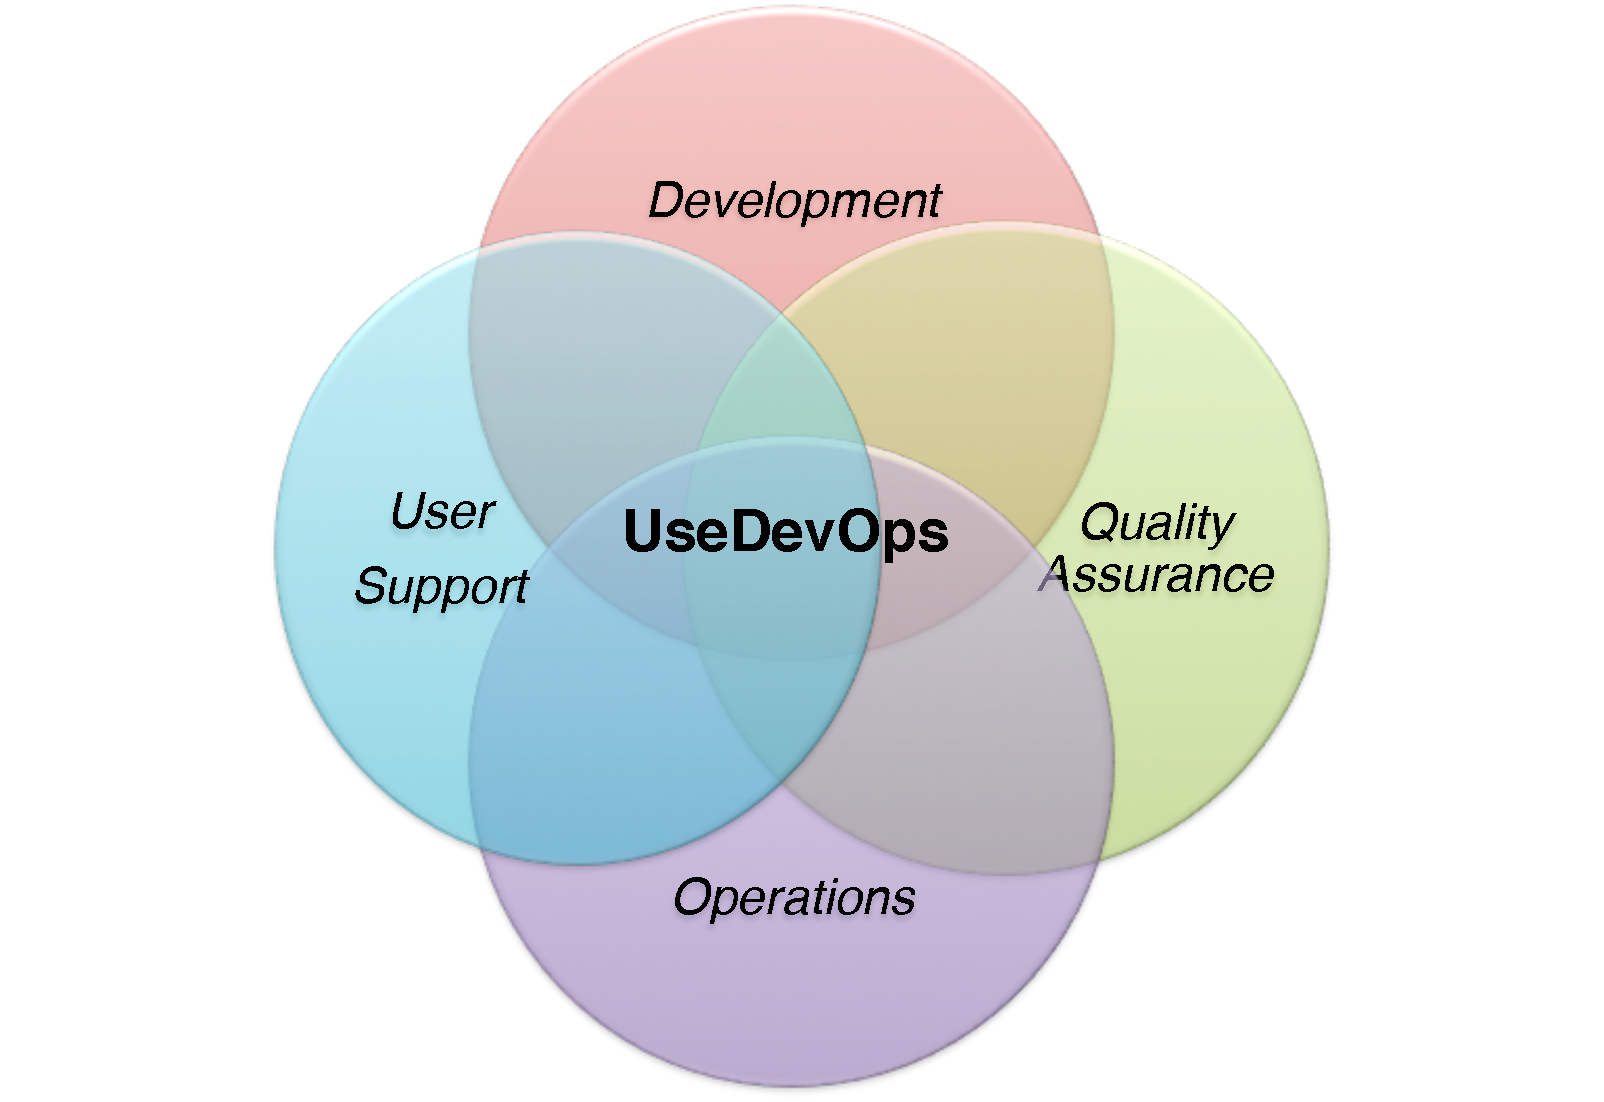
\includegraphics[width=0.5\textwidth]{images/usedevops.pdf}
  \caption{User Support integrated into DevOps leads to UseDevOps.}
  \label{F:usedevops}
\end{figure}


\subsection{Support for Education}

To support the many educational and research projects on FutureGrid we have provided through a portal significant amount of material on how to use the discussed services. In addition, we realized that not every educational project has users with advanced computer experience and we hence provide for such projects the ability to a streamlined user interface rather than having the users fight with complex command line syntax and parameters. For example, we provided for a recent MOOC on big data taught with resources on FutureGrid the basic functionality not only to start VMs as part of the IaaS framework, but also to deploy sophisticated images that contain preinstalled software and allow services to be hosted by the users such as iPypthon, R and much more. This was implemented on top of OpenStack while utilizing the newest OpenStack services such as heat. The management of the VMs and starting of the iPython server was controlled by a python application that provides the user with a menu system. Thus the management of them became literally, as easy as pressing 1, 2, 3, ... in the menu. For other classes we also have provided completely separate OpenStack deployments as the teachers were afraid that students would not have enough resources due to the shared environment. However we learned from this that the teachers overestimated the actual utilization of the project and many resources were not used. Based on this analysis we do now have a model to justify the creation of more relaxed access policies and can justify that even classes should be provided in the main region that FG provides. If resource contention would become an issue we could set aside a special region for a limited number of time. Reconfiguration needs have also arisen where one day a class may want o explore traditional MPI, while the next they want to experiment with Hadoop. Furthermore, we identified that several users wanted to combine various cloud IaaS platforms in order to avoid resource overprovisioning, or were interested in combining all resources. 



\FILE{cloudmesh.tex}

\section{Cloudmesh}\label{S:cloudmesh}

At \cite{github-cloudmesh}we find an extensive set of information about cloudmesh that is cited within this section. 
From the experience with FutureGrid we identified the need for a more tightly integrated software infrastructure addressing the need to deliver a software-defined system encompassing virtualized and bare-metal infrastructure, networks, application, systems and platform software with a unifying goal of providing Cloud Testbeds as a Service (CTaaS). This system is termed cloudmesh to symbolize 

\begin{enumerate}[(a)]

\item the creation of a tightly integrated mesh of services targeting multiple IaaS frameworks 

\item the ability to federate a number of resources from academia and industry. This includes existing FutureGrid infrastructure, Amazon Web Services, Azure, HP Cloud, Karlsruhe using not only one IaaS framework but various. 

\item the creation of an environment in which it becomes more easy to experiment with platforms and software services while assisting to deploy them more easily.  

\end{enumerate}

In addition to virtual resources, FutureGrid exposes bare-metal provisioning to users, but also a subset of HPC monitoring infrastructure tools. Services will be available through command line, API, and Web interfaces.

\subsection{Functionality}

Cloudmesh provides due to its integrated services the ability to be an onramp for other clouds. It also provides information services to various system level sensors to give access to sensor and utilization data. They internally can be used to optimize the system usage. The provisioning experience from FutureGrid has taught us that we need to provide the creation of new clouds, the repartitioning of resources between services (cloud shifting), and the integration of external cloud resources in case of over provisioning (cloud bursting). As we deal with many IaaS we need an abstraction layer on top of the IaaS framework. Experiment management is conducted with workflows controlled in shells \cite{cmd3}, Python/iPython, as well as systems such as OpenStack?s Heat, Accounting is supported through additional services such as user management and charge rate management. Not all features are yet implemented. Figure \label{F:cm-func} shows the main functionality that we target at this time to implement.

\begin{figure}[htb]
  \centering
    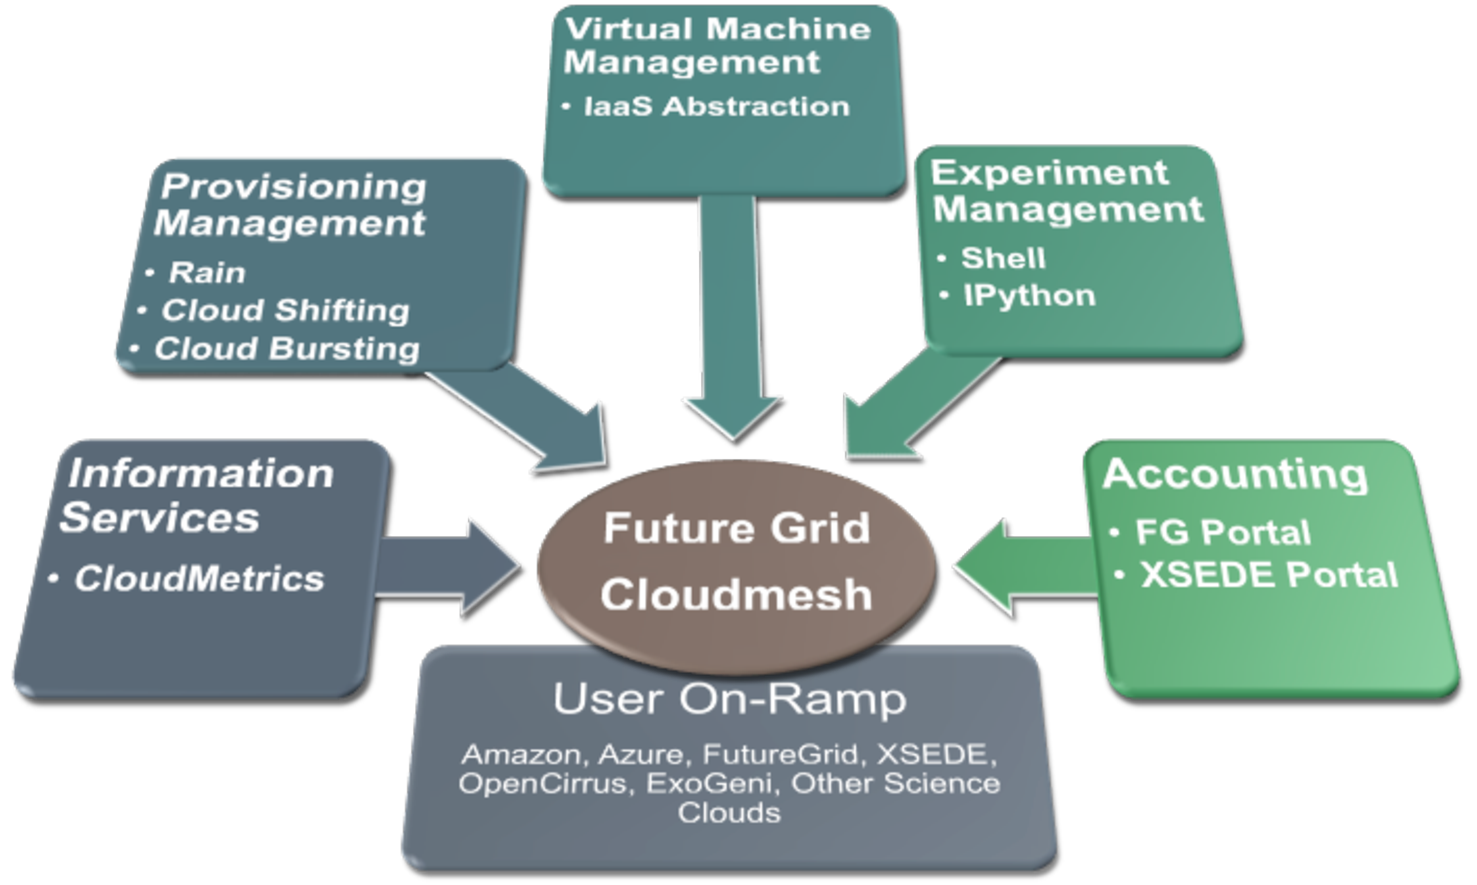
\includegraphics[width=1.0\textwidth]{images/cm-functionality.pdf}
  \caption{CM Functionality.}\label{F:cm-func}
\end{figure}


\subsection{Architecture}

The three layers of the Cloudmesh architecture include a Cloudmesh Management Framework for monitoring and operations, user and project management, experiment planning and deployment of services needed by an experiment, provisioning and execution environments to be deployed on resources to (or interfaced with) enable experiment management, and resources.

\begin{figure}[htb]
  \centering
    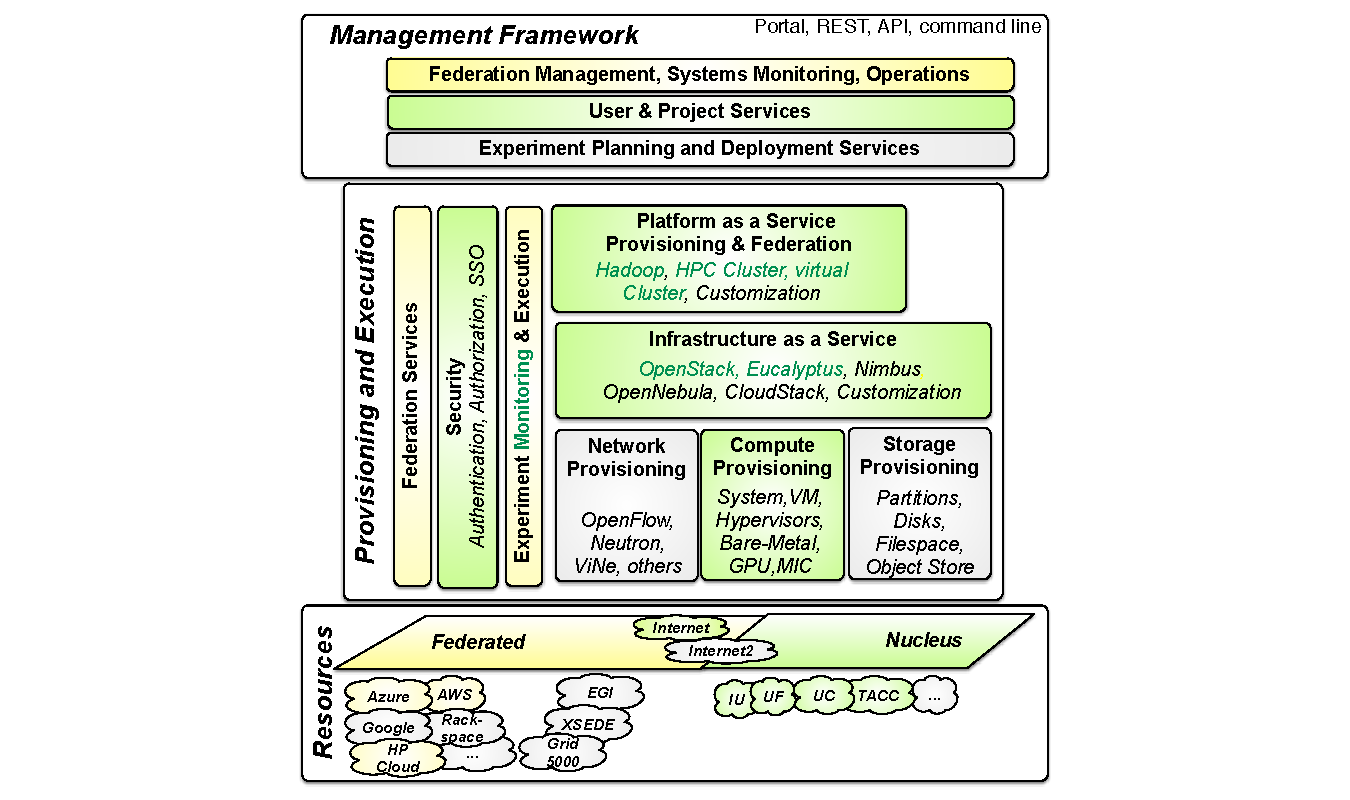
\includegraphics[width=1.0\textwidth]{images/cm-arch.pdf}
  \caption{CM Architecture.}
\end{figure}

\paragraph{System Monitoring and Operations.}

The management framework contains services to facilitate FutureGrid day-to-day operation, including federated or selective monitoring of the infrastructure. Cloudmesh leverages FutureGrid for the operational services and allows administrators to view ongoing system status and experiments, as well as interact with users through ticket systems and messaging queues to inform subscribed users on the status of the system.
The cloudmesh management framework offers services that simplify integration of resources in the FutureGrid nucleus or through federation. This includes, for user management, access to predefined setup templates for services in enabling resource and service provisioning as well as experiment execution. To integrate IaaS frameworks cloudmesh offers two distinct services:

(a) a federated IaaS frameworks hosted on FutureGrid,
(b) the availability of a service that is hosted on FutureGrid allowing the integration of IaaS frameworks through user credentials either registered by the users or automatically obtained from our distributed user directory.

For (b) several toolkits exist to create user-based federations, including our own abstraction level which supports interoperability via libcloud, but more importantly it supports directly the native OpenStack protocol and overcomes limitations of the EC2 protocol and the libcloud compatibility layer. Plugins that we currently develop will enable access to clouds via firewall penetration, abstraction layers for clouds with few public IP addresses and integration with new services such as OpenStack Heat. We successfully federated resources from Azure, AWS, the HP cloud, Karlsruhe Institute of Technology Cloud, and four FutureGrid clouds using various versions of OpenStack and Eucalyptus. The same will be done for OpenCirrus resources at GT and CMU through firewalls or proxy servers.
Additional management flexibility will be introduced through automatic cloud-bursting and shifting services. While cloud bursting will locate empty resources in other clouds, cloud shifting will identify unused services and resources, shut them down and provision them with services that are requested by the users. We have demonstrated this concept in 2012 moving resources for more than 100 users to services that were needed based on class schedules. A reservation system will be used to allow for reserved creation of such environments, along with improvements of automation of cloud-shifting.

\paragraph{User and Project Services}

FutureGrid user and project services simplify the application processes needed to obtain user accounts and projects. We have demonstrated in FutureGrid the ability to create accounts in a very short time, including vetting projects and users – allowing fast turn-around times for the majority of FutureGrid projects with an initial startup allocation. Cloudmesh re-uses this infrastructure and also allows users to manage proxy accounts to federate to other IaaS services to provide an easy interface to integrate them.

\paragraph{Accounting and App Store}

To lower the barrier of entry Cloudmesh will be providing a shopping cart which will allow checking out of predefined repeatable experiment templates. A cost is associated with an experiment making it possible to engage in careful planning and to save time by reusing previous experiments. Additionally, the Cloudmesh App Store may function as a clearing-house of images, image templates, services offered and provisioning templates. Users may package complex deployment descriptions in an easy parameter/form-based interface and other users may be able to replicate the specified setup with.
Due to our advanced Cloudmesh Metrics framework we are in the position to further develop an integrated accounting framework allowing a usage cost model for users and management to identify the real impact of an experiment on resources. This will be useful to avoid overprovisioning and inefficient resource usage. The cost model will be based not only on number of core hours used, but also the capabilities of the resource, the time, and special support it takes to set up the experiment. We will expand upon the metrics framework of FutureGrid that allows measuring of VM and HPC usage and associate this with cost models. Benchmarks will be used to normalize the charge models.

\paragraph{Networking.}

in{ceWe have a broad vision of resource integration in FutureGridources be with systems offering different levels of control from bare metal to use of a portion of a resource. Likewise, we must utilize networks offering various levels of control, from standard IP connectivity to completely configurable SDNs as novel cloud architectures will almost certainly leverage NaaS and SDN alongside system software and middleware. FutureGrid resources will make use of SDN using OpenFlow whenever possible and the same level of networking control will not be available in every location.

\paragraph{Monitoring.}

To serve the purposes of CISE researchers, Cloudmesh must be able to access empirical data about the properties and performance of the underlying infrastructure beyond what is available from commercial cloud environments. To accommodate this requirement we have developed a uniform access interface to virtual machine monitoring information available for OpenStack, Eucalyptus, and Nimbus. In the future, we will be enhancing the access to historical user information. Right now they are exposed through predefined reports that we create on a regular basis. To achieve this we will also leverage the ongoing work while using the AMPQ protocol. Furthermore, Cloudmesh will provide access to common monitoring infrastructure as provided by Ganglia, Nagios, Inca, perfSonar, PAPI and others.


\subsection{Cloud Shifting}

We have already demonstrated via the RAIN tool in cloudmesh that it is possible to easily shift resources between services. We are currently expanding upon this idea and developing more easy to use user interfaces that assist administrators and users through role and project based authentication to move resources from one service to another (see Figure \ref{F:shift}).

\begin{figure}[htb]
  \centering
    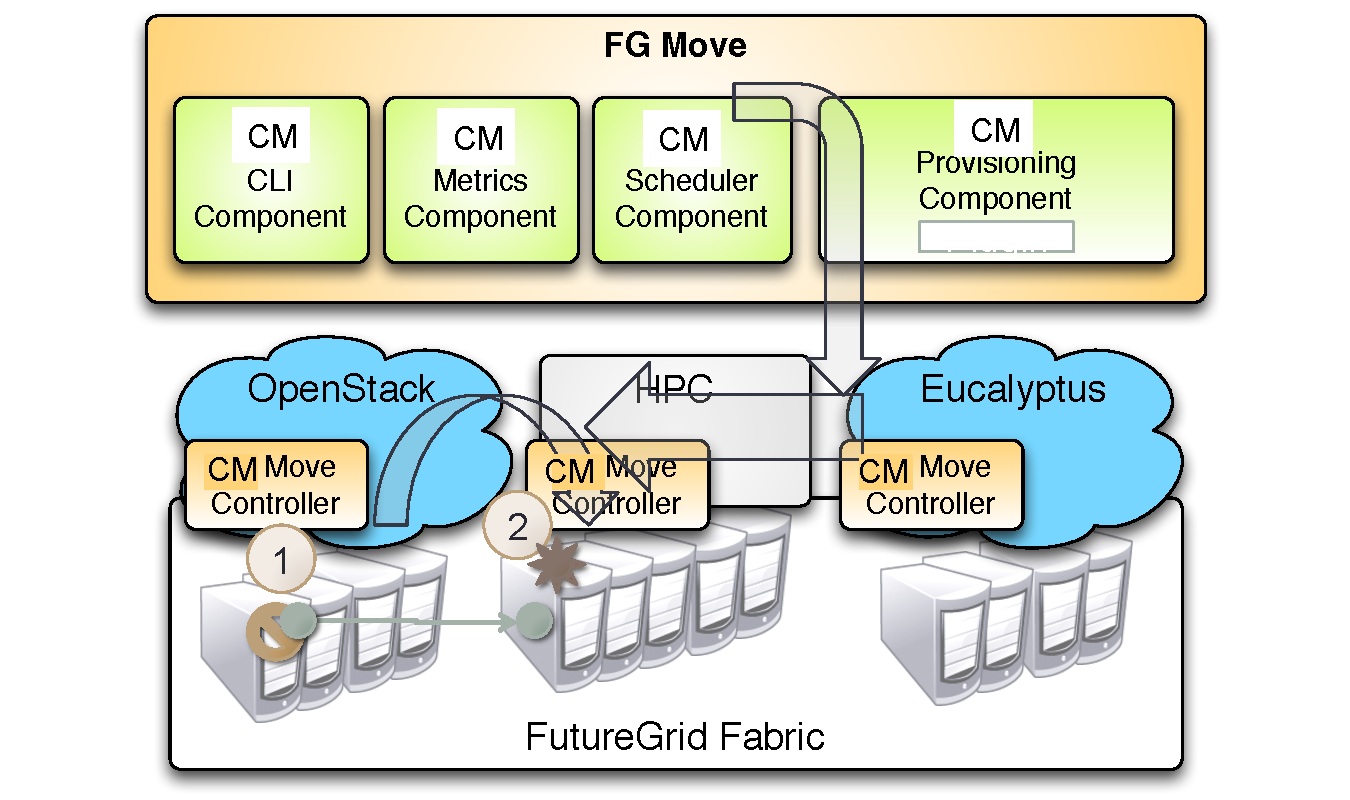
\includegraphics[width=0.75\textwidth]{images/shift2.pdf}
  \caption{Shifting resources makes it possible to offer flexibility
    in the service distribution in case of over or underprovisioning.}\label{F:shift}
\end{figure}

\subsection{Graphical User Interface}

Despite the fact that cloudmesh was originally a quite sophisticated command shell and command line tool, we have spend recently more time in exposing this functionality through a convenient Web interface. Some more popular views if this interface are depicted in Figure \ref{F:instances} hinting on how easy it is with a single button to create multiple VMs across a variety of IaaS. Also nice is that this not only includes resources at IU but also at external locations. Pushing this easy management in a more sophisticated experience for the user while associating one-click deployments that include the ability to deploy virtual clusters, Hadoop environments, and other more elaborate setups we provide an early prototype screenshot in Figure \ref{F:oneclick}.

\begin{figure}[htb]
  \centering
    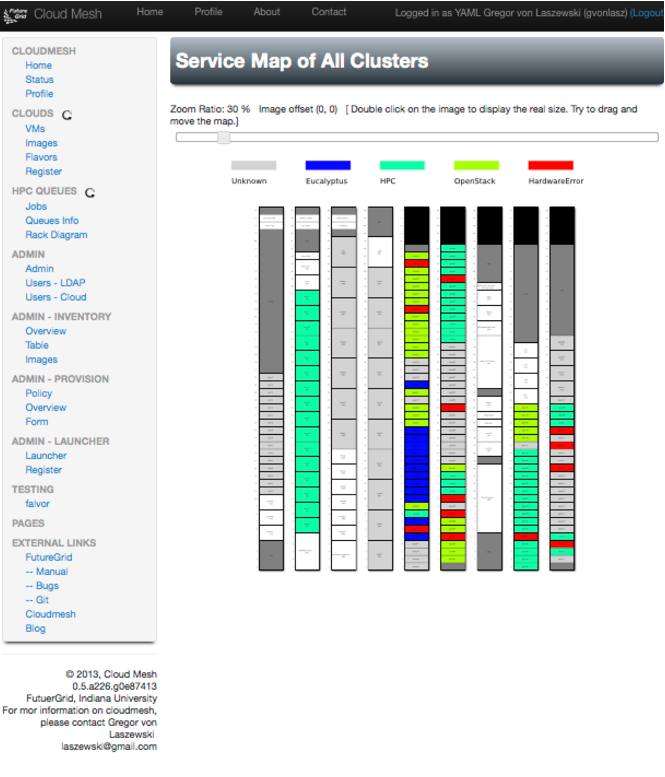
\includegraphics[width=.7\textwidth]{images/rainbow.pdf}
  \caption{Monitoring the Service distribution of FutureGrid with cloudmesh.}
\end{figure}

\begin{figure}[htb]
  \centering
    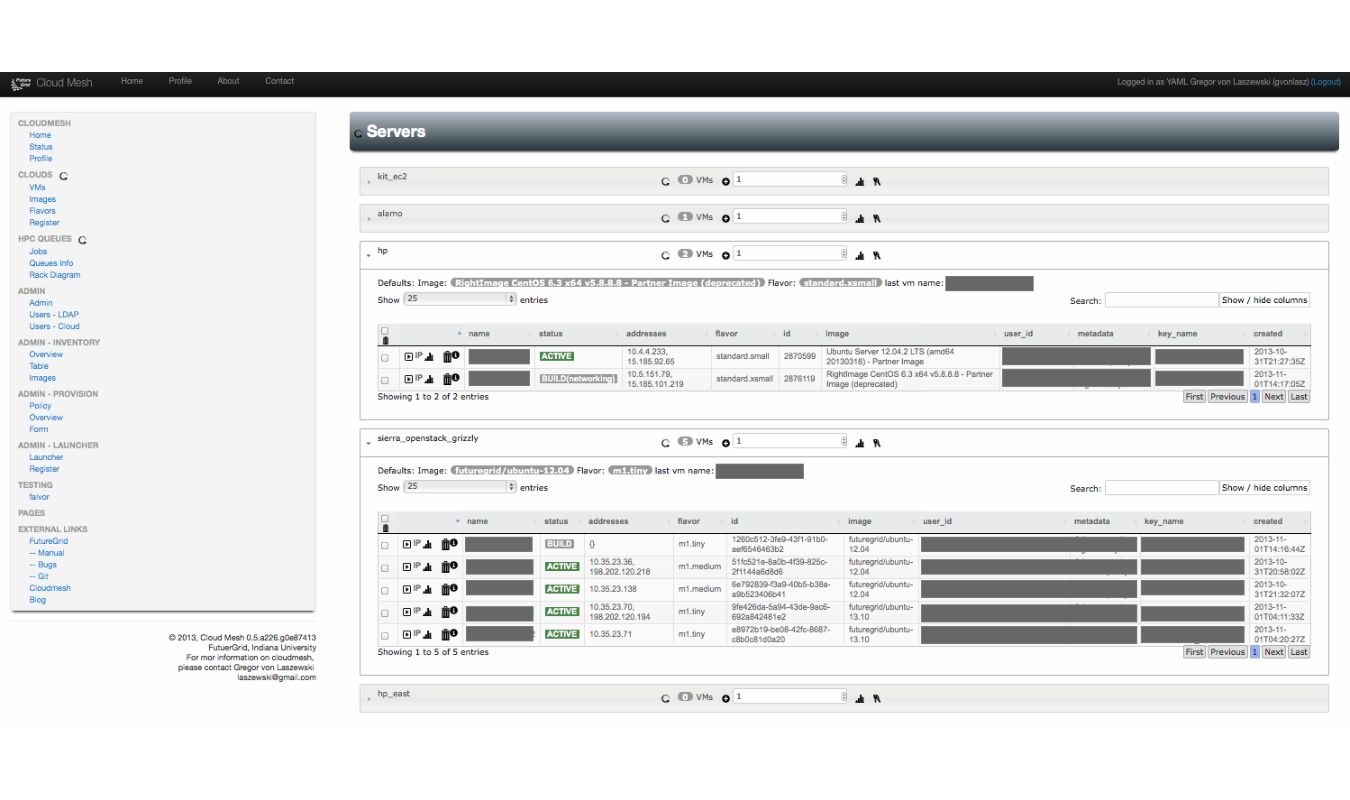
\includegraphics[width=.9\textwidth]{images/instances.pdf}
  \caption{Rainbow.}\label{F:instances}
  \centering
    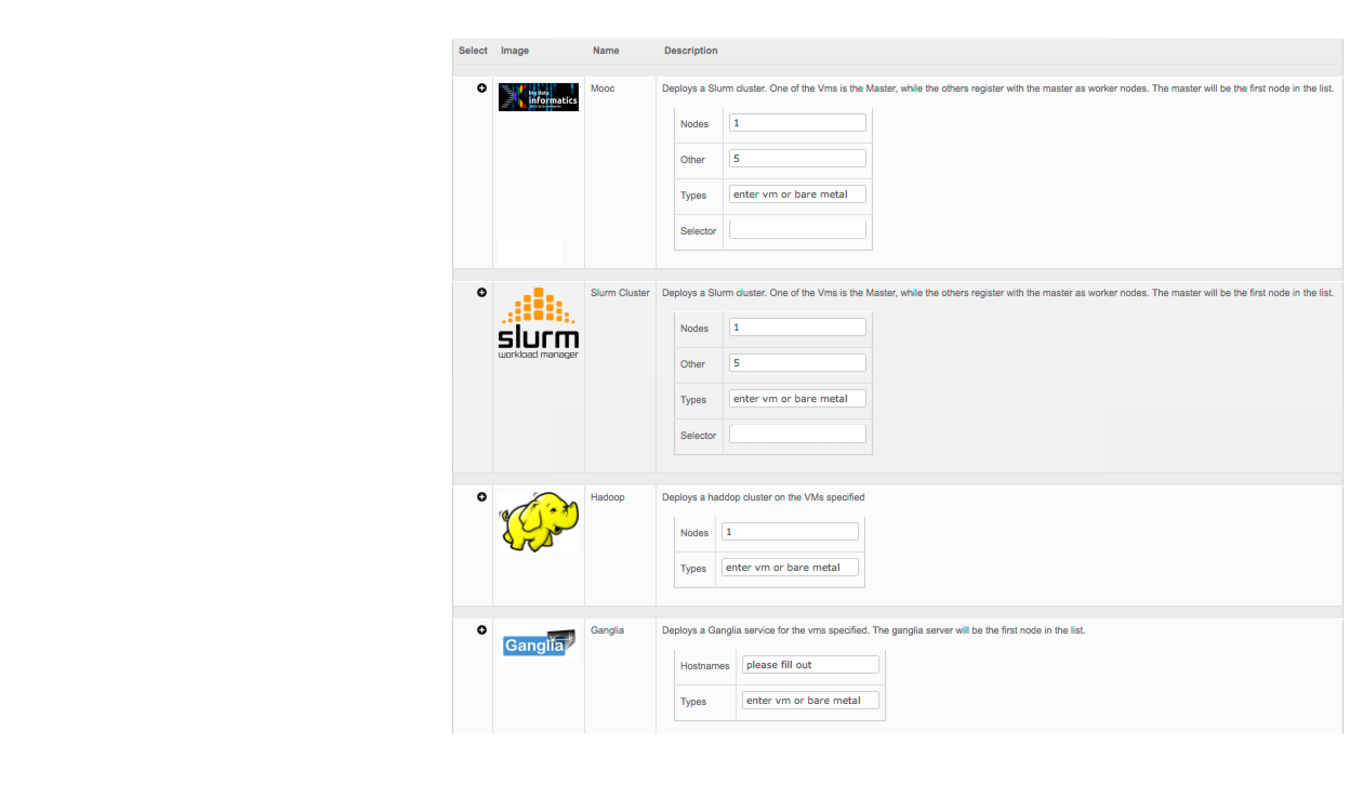
\includegraphics[width=.9\textwidth]{images/oneclick.pdf}
  \caption{One click deployment of platforms and sophisticated
    services that could even spawn multiple resources.}\label{F:oneclick}
\end{figure}


\afterpage{\clearpage}

\section{Summary}\label{S:summary}

In this chapter we have described FutureGrid and focused on services that are beneficial for big data analysis. Based on the discussion it is clear that such a system is extremely complex but provides many benefits of offering multiple services within the same infrastructure. Performance experiments can thus be not only conducted while conducting big data analysis in virtual machines, but on a variety of IaaS and PaaS environments. Moreover these experiments can directly be compared to bare metal provisioned services. Hence, users can evaluate what impact such technologies have on their codes. Comparisons of different programming frameworks can be achieved and future activities in regards to efficiency and usability can be deducted. The lessons learned from FutureGrid are motivating a toolkit cloudmesh that already today allows to manage virtual machines on a avriety of infrastructure as a service frameworks. The easy deployment of sophisticated setups with a one click deployment has been validated as part of an infrastructure designed for a MOOC. Furthermore the novel concept of shifting resources \cite{las08federated-cloud} between services to support services that need more resources is a significant contribution by cloudmesh. Image management and creation under security restrictions \cite{fg-1295} is furthermore an important aspect. We will continue to develop the cloudmesh environment and make it available to our users.


\section*{Acknowledgement}

Some of the text published in this chapter is available form the FutureGrid portal. The FutureGrid project is funded by the National Science Foundation (NSF) and is led by Indiana University with University of Chicago, University of Florida, San Diego Supercomputing Center, Texas Advanced Computing C research \cite{las12fg-bookchapter}. The Futurenter, University of Virginia, University ofrid has a limited amount of storage space and us Tennessee, University of Southern California, Dresden, Purdue University, and Grid 5000 as partner sites. This material is based upon work supported in part by the National Science Foundation under Grant No. 0910812. If you use FutureGrid and produce a paper or presentation, we ask you to include the reference \cite{las2010gce,las12fg-bookchapter}.

\bibliographystyle{IEEEtranS}
\bibliography{%
bib/references,%
bib/vonLaszewski-jabref,%
bib/image-refs,%
bib/cyberaide-cloud,%
bib/python}

%%%%%%%%%%%%%%%%%%%%%%%%%%%%%%%%%%%%%%%%%%%%%%%%%%%%%%%%%%%%
%\clearpage

%\appendix

%\FILE{overview.tex}

\section{Overview}

FutureGrid is a national-scale Grid, Cloud and HPC computing test-bed service of modest size that includes a number of computational resources at five distributed locations. FutureGrid experience and architecture is built around software defined systems at all levels of the stack shown in figure – encompassing VM and bare-metal infrastructure, networks and application, systems and platform software – with a unifying goal of providing Computing Testbeds as a Service. FutureGrid systems total 4704 cores divided into distributed general purpose clusters at Chicago, Florida, IU and TACC; a Cray XT5m at IU and four small specialized clusters supporting SSD (at SDSC), Large Disk Large memory (at IU) and NVIDIA GPU’s (IU). FutureGrid’s system model has grown in sophistication and now supports software-defined systems – encompassing virtualized and bare-metal infrastructure, networks, application, systems and platform software – with a unifying goal of providing Cloud Testbeds as a Service (CTaaS). Cloudmesh aggregates resources not only from FutureGrid, but also from OpenCirrus, Amazon, Microsoft Azure, and HP Cloud and GENI resources. Cloudmesh was originally developed in order to simplify the execution of multiple concurrent experiments on a federated cloud infrastructure and in addition to virtual resources, FutureGrid exposes bare-metal provisioning to users.

Users can apply for projects either at FutureGrid or XSEDE portals. A single account provides a user access to all FutureGrid machines and we can describe the type of work that can be done by looking at FutureGrid’s experience based on 3 and a half years of operation with 355 projects and 2178 users from 55 countries with 76\% from the USA. 51.8\% of these projects were mainly computer science (including middleware and cyberinfrastructures) research, 9.6\% technology evaluation, 13.2\% education, 9.6\% in life sciences and 11.5\% in other application domains. We looked in detail at the last 200 projects starting October 25 2011 to understand in more detail usage paradigms. 98 of these projects needed only virtual machine (VM) access and 54 requested both virtualized and non-virtualized nodes. Of the 48 projects not requesting VM’s, 8 were studying cloud technology like Hadoop and so 160 projects (80\%) were cloud related. 16 projects involved GPU access and 30\% of all projects used MapReduce in some way. The use of FutureGrid for education has been increasing and 21\% of projects in last 2 years have been for education dividing into 29 semester length classes and the 13 remaining split between REU training, Summer Schools, Tutorials, and workshops. Of 42 education requests, 36 were computer science, 3 application oriented and 3 mixed. These education classes covered areas like cloud computing, distributed systems, parallel computing, big data, data-intensive computing and datamining, business analytics, autonomic computing, cyberinfrastructure, storage, software carpentry, data centers and large scale infrastructure, MapReduce, high performance computing, networking, science clouds, and particular tools supported on FutureGrid.
Coming to the 136 research projects, 109 had a major CS component and 44 an application component with 17 of these jointly classified. Application projects included 18 from bioinformatics including genomics, radiology, cardiovascular simulation, surgery control, health sensors, iPlant cyberinfrastructure and text mining. Only 10 application projects had a simulation (major focus of most HPC systems) focus including combustion, CFD, subsurface modeling, climate, weather, ocean, environment, earthquakes and supply chains. Physical science and engineering data intensive applications (8 projects) include astronomy, particle physics, aerospace reliability, ocean observation, hydroinformatics, GIS and accelerator control. 6 social science projects include conflict resolution, disaster management using Twitter, optimization, political science and economics.

Turning to CS related projects, 23 were in basic virtualization (IaaS) areas. They included provisioning, deployment, new hypervisors including increased performance, elasticity and scheduling, resource management, benchmarking, emulation, and IaaS scaling to support MOOC’s. 4 projects studied distributed clouds and storage with federation. 3 projects centered on networking (routing, optimized devices and emulation) and 2 studied software engineering for clouds. 5 projects were aimed at cyberphysical systems with health, power and mobile applications and FutureGrid used for control and support analytics. 2 projects had a P2P focus covering security and fault tolerance. Security was popular with 10 projects covering trusted P2P storage, mobile and other clients, intrusion detection, file sharing, confidentiality and integrity of data, vulnerability, watermarks and hybrid clouds with different security models. There were 4 HPC programming language projects and 8 covering cloud programming with scheduling, fault tolerance and runtime. 5 fault tolerance projects covered P2P, MapReduce, workflow and HPC. 4 projects covered distributed software transactional memory and concurrency control. Data systems were very popular with 13 projects covering cloud storage, data transfer, NoSQL, streaming big data, Apache software stack, analytics, image retrieval, testing, provenance and the semantic web. 2 projects studied enterprise software issues. 9 artificial intelligence projects covered learning networks for images and social media, large scale image classification by clustering, machine learning, text mining, and agents. Network science with 3 projects saw use of NoSQL datastores to study Twitter, a major infrastructure to support graph and other tools and community detection. Finally 13 projects focused on cyberinfrastructure middleware with XSEDE and EMI (European Middleware initiative) systems, software as a service for HPC simulations, HPC clouds, MPI porting, fault tolerance, workflow, scheduling and resource management, tools, logging and performance.
There were 19 Evaluation projects which covered XSEDE testing (a major actual and intended use of FutureGrid), Open Science Grid testing, particle physics, Apache Big Data stack, Solid State disks, comparison of different VM frameworks, familiarization with cloud technology, GPU’s and studies aimed at planning institutional initiatives in cloud computing. There were 3 Interoperability projects involving long term support of standard end-points. 

FutureGrid interacts with XSEDE on integrating accounting approaches, EOT and software testing.


\end{document}


